\documentclass[11pt,a4paper, twoside, openright]{memoir}

\usepackage{PhDstyle}

\usepackage{algpseudocode,algorithm,algorithmicx}

\newcommand*\Let[2]{\State #1 $\gets$ #2}
\algrenewcommand\algorithmicrequire{\textbf{Precondition:}}
\algrenewcommand\algorithmicensure{\textbf{Postcondition:}}

\def\rightarrowfill@@{\arrowfill@@\relax\relbar\rightarrow}


\addbibresource{switches_ref.bib}

\begin{document}
\title{Using computational modelling to build robust synthetic genetic switches}
\author{Miriam Leon \\ Supervisor: Chris P Barnes\\ Department of Cell and Developmental
 Biology \\ University College London}
\date{}
\maketitle

%\newpage
%\section{Declaration}

%I, Miriam Leon, confirm that the work presented in this thesis is my own. Where information has been derived from other sources, I confirm that this has been indicated in the thesis.

\newpage
\section{Abstract}
Creating synthetic devices that are robust to changing cellular contexts will be key to the success of 
synthetic biology. When faced with a set of competing designs for a given genetic circuit one is likely 
to choose the simplest possible model that can achieve the desired behaviour. However simple systems are 
often the least robust and it is known that additional feedback interactions can increase robustness to 
extrinsic noise sources. The genetic toggle switch is examined, consisting of two mutually repressing 
transcription factors. It is known for exhibiting bistability, and is found in natural systems when 
binary fate decisions need to be made, such as in a developmental pathway. It can also be used in 
synthetic systems to sense and respond to different environments.
\noindent
Here a new tool is presented, called StabilityChecker, that takes advantage of sequential Monte Carlo to 
identify regions of parameter space capable of producing the desired stability while handling uncertainty 
in biochemical rate constants and initial conditions. StabilityChecker is tested against known systems. A 
collection of networks are examined, ranging from the simple genetic toggle switch to those containing different 
positive feedback connections. 
\noindent
We verify StabilityChecker against known results of the simple toggle switch. We find that positive feedback 
and other regulatory interactions can significantly increase the robustness of these switching systems. 


\newpage
\setcounter{secnumdepth}{3}
\setcounter{tocdepth}{3}
\tableofcontents* 
\newpage
\listoffigures
\newpage
\listoftables
\pagestyle{plain}

%% --------------------------------------------------------------
%% CHAPTERS
%% --------------------------------------------------------------

%% Introduction -----------------------------------------------%%
%\mainmatter*
%chapter{Introdution}

%% StabilityChecker -------------------------------------------%%
\mainmatter*
\chapter{Modelling switches}
\section{Introduction}

A challenge that synthetic biology is facing is the ability to build synthetic devices that are robust to changing cellular contexts. Unknown initial conditions and parameter values as well as the variability of the cellular environment, extracellular noise and crosstalk makes the majority of synthetic genetic devices non-functional \autocite{Chen:2009ea}. There has been a great progress in the  quantity and quality of devices being created(), but we are still lagging behind in our ability to rationally design a device and minimize the time-consuming and expensive experimental trial and error. 

One of the most common devices used in synthetic biology is the genetic toggle switch. A toggle switch consists of a set of transcription factors that mutually repress each other \autocite{Gardner:2000vha}. Toggle switches play a major role in binary cell fate decisions like stem cell differentiation, as they are capable of exhibiting bistable behaviour. Bistability is defined as the system being able to have two distinct phenotypic states but no intermediate state. Bistability is a property that is important in nature and a valuable resource to tap into in synthetic biology. It allows cells to alter their response to environmental cues and increases the overall population fitness by 'hedge-betting' the response of the population.

Bistability ensures that the differentiating cell will go down one pathway, or the other, with no intermediate phenotypes being possible. This is vital for the correct development of a cell in a specific pathway. One example is the trophectoderm differentiation pathway, in which a mutually inhibitory toggle switch exists between Oct3/4 and Cdx2. This determines whether an Embryonic Stem cell will differentiate into a Trophectoderm cell, if Cdx2 dominates the system, or an Inner Cell Mass cell if Oct3/4 dominates \autocite{Niwa:2005fz}. Bistability is critical in this system as a cell must differentiate into either a trophectoderm cell or an inner cell mass cell, thus the signal to do so must be straightforward. In the case of the GATA1 and PU.1 toggle switch, the transcription factor pair controls the fate of the common myeloid progenitors, and the two possible differentiation paths are erythroid and myeloid blood cells \autocite{Chickarmane:2009by}. The double-negative feedback loop created by the mutually repressive pair of transcription factors sustains the system in balance until an external stimulus causes one of the two transcription factors to increase in concentration. The increased concentration of one transcription factor causes the increased repression of the production of the antagonistic transcription factor, tipping the balance towards the dominance of the first transcription factor. The double negative feedback loop reinforce this dynamic and the system remains in the same state, until an external stimulus disturbs it \autocite{FerrellJr:2002fh}.

Despite their simplicity, toggle switches can be powerful building blocks with which to create complex responses in a synthetic network. They have been used in isolation() or in tandem to create complex networks and signalling cascades. 

The toggle switches have been studied extensively and there are numerous studies based on a number of different methods of modelling and analysing the dynamics of this system. Numerous studies have concluded that cooperativity is a necessary condition for bistability to arise (). \textcite{Lipshtat:2006wb} found that stochastic effects can give rise to bistability even without cooperativity in three kinds of switch: In the exclusive switch, in which there can only be one repressor bound at any one time, the switch in which there is degradation of bound repressors or the switch in which free repressor proteins can form a complex which renders them inactive as transcription factors \autocite{Lipshtat:2006wb}. In their study, \textcite{Ma:2012dt} found that the stochastic fluctuation in a system involving such a small number of molecules, like the toggle switch, uncovers effects that can not be predicted by the fully deterministic case. In their system, the toggle switch was found to be tristable, as small number effects render the third unstable steady state stable. In the study conducted by \textcite{Biancalani:2015vy}, they identified multiplicative noise as the source of bistability in the stochastic case. This bistability disappears of the noise source is reduced below a threshold, which in the toggle switch is represented by the repression strength. Thus if the repression strength falls below a certain threshold, the switch becomes monostable. In the genetic toggle switch the source of noise is the weakness of the repression so thus, increasing repression strength one decreases the source of noise and increases the stability of the switch \autocite{Warren:2005kea}. \textcite{Warren:2005kea} concluded that the exclusive switch is always more robust than the general switch, since the free energy barrier is higher. As is clear from above, there is yet to exist a consensus on the stability a switch is capable of, and the most appropriate method of modelling it. Different methods arrive at different conclusions, creating a confusion on which behaviour to be expected by the experimentalist for even a simple system like the toggle switch, consisting of just two genes. The toggle switch cannot be used as a building block of a bigger, more complex system, until its behaviour can be predicted otherwise designing such a system with predictable behaviour will be near impossible.

In order to solve this problem, we created a framework, StabilityChecker, that can be used to elucidate the stability each model is capable of, under conditions of parameter uncertainty. Using this framework one can study the different methods of modelling the switch and be able to attribute the differences in the results to each type of modelling. By using the same framework to compare the different modelling techniques we can get to the bottom of what the stability the switch is capable of and why each method produces a different result. We will use StabilityChecker to study three different models of the toggle switch. This methodology can also be used to uncover the design principles behind making a bistable switch, as well as those necessary to make a tristable switch. The methodology presented here can be used to study existing systems, toggle switches that exist in nature, as well as synthetic systems, if used as an aid to system design in synthetic biology. By identifying the parameter ranges that can give rise to the desired stability of a system, one can choose the parts of the genetic system accordingly. For example, if StabilityChecker dictates that gene expression must be low for a given stability, one can select a weak promoter or a low copy plasmid for their desired construct. 

% \autocite{Lipshtat:2006wb}
%To qualify as a switch the spontaneous switching rate must be much lower than the rates of the relevant processes in the cell.Numerous studies have concluded that cooperative binding is a necesasary condition for the emergence of the two distinct stable states (11,14)
%It was also observed that in the presence of cooperative binding stochastic effects contribute to the broadening of the parameter range which bistability occurs. 
%here show that stochastic effects enable bistability even without cooperative binding. Bistability takes place even when active proteins appear in high copy numbers.
%in the exclusive switch stochastic effects give rise to bistability even without cooperativity between transcription factors. Weak repression -> monostable, strong repression -> bistable. deadlock situation is impossible.
%bistability without cooperative binding: exclusive switch, degradation of bound repressors, free A and B proteins may form a complex which is not active as a transcription factor. 
%
% \autocite{Ma:2012dt}
%stochastic fluctuation is not negligible in such a small system
%a few simulational works having captured some new kinetic stability via KMC simulations including multi-stability. Experimentally and theoretically revealed an additional kinetic stable state nearby the traditionally regarded USS. The whole system could be from monostable to tristable under different conditions.  Source of additional kinetic stability: the discrete and fluctuate nature of molecule numbers, especially when they are often very close to or equal to zero.
%these are composite effects presented in small reaction systems that have pivotal molecules fluctuating on the verge of extinction.
%The results show that the behaviour of such a small system is quite different from what a fully deterministic model could predict. Besides fluctuation, there must be some features inherent in such a small system that contribute to the additional kinetic stability. it is the combined effects of the discrete, fluctuate, and non-negative features of molecular numbers in such a small system that result in the additional kinetic stability observed in experiments.
%
% \autocite{Lu:2014kc}
%Noise has been shown before to have a significant role in gene expression transitions and stability (9,10)
%Study effect of white Gaussian noise and shot noise on the dynamics of multi-state switches
%The two-way switch has two stable fixed points and a saddle point and the three-way switch has three stable fixed points and two saddle points.
%
% \autocite{Strasser:2012kt}
%protein variations of a differentiating cell influence the dynamics of the decision-making process and lead to stochastic transitions between the two steady states.
%probabilistic models of the toggle switch account for low copy numbers and intrinsic fluctuations
%contrary to deterministic models transitions between the two macroscopic regimes where one of the two genes dominates are possible due to the inherently noisy gene transcription even without cooperative binding of transcription factors.
%the inclusion of both mRNA and protein leads to an interesting change in system dynamics. the probabilistic two stage description exhibits complex multi-attractor dynamics without auto-activation and cooperativity. 
%assume monomeric transcription factor binding.
%Four attractors
%
% \autocite{Warren:2005kea}
%switch stability is decreased by phenomena that increase the noise in gene expression
%robustness against biochemical noise can be drastically enhances if switch is mutually exclusive
%Natural examples in lambda phage and human herpesvirus3. synthetic switches also constructed in vivo (9)
%switches usually flipped by external signals
%often so stable that they remain in one state until external trigger flips it. in lambda phage a spontaneous flip occurs as low as 10(to the)12 s (8). 
%region of bistability significantly larger for exclusive switch than that for general switch
%while the kinetic prefactor is toughly the same for both switches, the free energy barrier for flipping is significantly higher for the exclusive switch than for the general switch. 
%
% \autocite{}
%citation = Biancalani 
%Cooperative binding, more than a single TF can bind the DNA SEQUENCE AND THE BINDING PROBABILITY DEPENDS ON WHETHER there are molecules already bound to the sequence. (15) bimodality reported in a synthetic budding yeast system which concluded that the bimodal behaviour is induced by mRNA noise
%(11)(14) genetic toggle switch bimodal behaviour due to demographic noise even in the absence of cooperative binding.
%Here tehy show that bimodality is induced by multiplicative noise: the noise strength vanishes at the bimodal states whereas it is maximal at the single stable fixed point. Bimodal behaviour ceases to occur if the noise strength in the system is reduced below a critical threshold. In genetic toggle switches noise is controlled by the repression strength. 
%
% \autocite{}
%citation = Wang 2007
%
%A system is termed bistable if it can switch between two distinct stable steady states but cannot rest in intermediate states under the excitation of external stimuli. Bistable systems are building blocks of larger regulatory elements: geentic networks and signalling cascades.
%Noise exists extensively in biological systems with a small number of molecules due to the intrinsically stochastic nature of biochemical reactions involved or because of environmental fluctuations.
%Since living systems are usually optimized to function in the presence of stochastic fluctuations(23) the biochemical networks must withstand considerable variations and random perturbations of biochemical parameters (24)
%Here show that in the case of the toggle switch the multiplicative noises resulting from stochastic fluctuations in degradation rates can induce switching
%
% \autocite{}
%citation = Siegal-Gaskins 2015
%Sturn's theorem from algebraic geometry
%dimer-dimer toggle switch is bistbale over a greater range of parameters then the monomer-dimer switch. There is no single parameter more improtant than any other for achieving bistability.
%
% \autocite{Chen:2012bd}
%Some tremendous challeneges still remain, how to rationally build genetic devices with predetermined erformance. One of the most used genetic devices is the toggle switch (2,7,15)
%Bistability confers cells the ability to stochastically switch between phenotyipic states to generate diversity in a population (17,18) but also makes it a core component of gene circuits for higher-level sequential logic processes such as adaptive learning (2,7,15)
%Here provide method for rational design of genetic toggle switches with predetermined bistability. Single postivie autoregulation
%establishes equivalence between RBS DNA sequence and its bistability. 

%-%-%-%-%-%-%-%-%-%-%-%-%-%-%-%%-%-%-%-%-%-%-%-%-%-%-%-%-%-%-%%-%-%-%-%-%-%-%-%-%-%-%-%-%-%-%%-%-%-%-%-%-%-%-%-%-%-%-%-%-%-%
%Why stability checker is useful
%
% \autocite{Toni:2009tr}
%In biological systems we lack reliable information about parameters
%In ABC methods, the evaluation of the likelihood is replaced by a simulation-based procedure (Pritchard et al. 1999; Beaumont et al. 2002; Marjoram et al. 2003; Sisson et al. 2007).
%information about sensitivity of the model to parameter variation.
%
%Let q be a parameter vector to be estimated. Given the prior distribution p(q), the goal is to approximate the posterior distribution, p(qjx)ff(xjq)p(q), where f(xjq) is the likelihood of q given the data x. 
%
%In ABC SMC, a number of sampled parameter values (called particles), {q(1), ., q(N )}, sampled from the prior distribution p(q), are propagated through a sequence of intermediate distributions, p(qjd (x0, x)ei), iZ1, ., TK1, until it represents a sample from the target distribution p(qjd (x0, x)eT). The tolerances ei are chosen such that e1O/OeTR0, thus the distributions gradually evolve towards the target posterior.
%
%
% \autocite{Barnes:2011hh}
%the modeling and model evaluation/characterization is incorporated directly into the design stage. 
%The statistical nature of the method has many attractive features including the handling of stochastic systems, the ability to perform model selection and the handling of parameter uncer- tainty in a well-defined manner.
% We used the ABC-SysBio and cuda-sim softwares (19, 35), which takes as input a set of SBML files and as such can be used by bioengineers and experimentalists to rationally com- pare their competing designs for a system. 






\section{Methods}

The algorithm we developed can be utilised to identify regions of parameter space capable of producing a desired stability while handling uncertainty in biochemical rate constants and initial conditions. It can be used to design new systems of desired stability or study the stability of existing systems. The method we are presenting here is based on the Approximate Bayesian Computation, Sequential Monte Carlo method, a statistical inference method developed by \textcite{Toni:2009tr}. This simulation-based method, using an iterative process can arrive at a distribution of parameter values that can give rise to a desired system behaviour. Given a prior distribution of values for each parameter in the model $\pi(\theta)$, and a desired behaviour, which in our case is model stability, can arrive at the posterior distributions $\pi(\theta|d(s_0, s*)\leq \epsilon_T)$. The tolerance $\epsilon$ represents the distance between the target behaviour and the current simulated behaviour. As this $\epsilon$ gradually becomes smaller, the distributions get nearer to the target distribution capable of giving rise to the desired behaviour \autocite{Toni:2009tr}. The advantages of this method is that it can handle stochastic as well as deterministic models, and can inherently handle parameter uncertainty \autocite{Barnes:2011hh}. The algorithm can be summarised as seen in Figure~\ref{fig:flowchart}.

\begin{figure}[p]
	\centering
	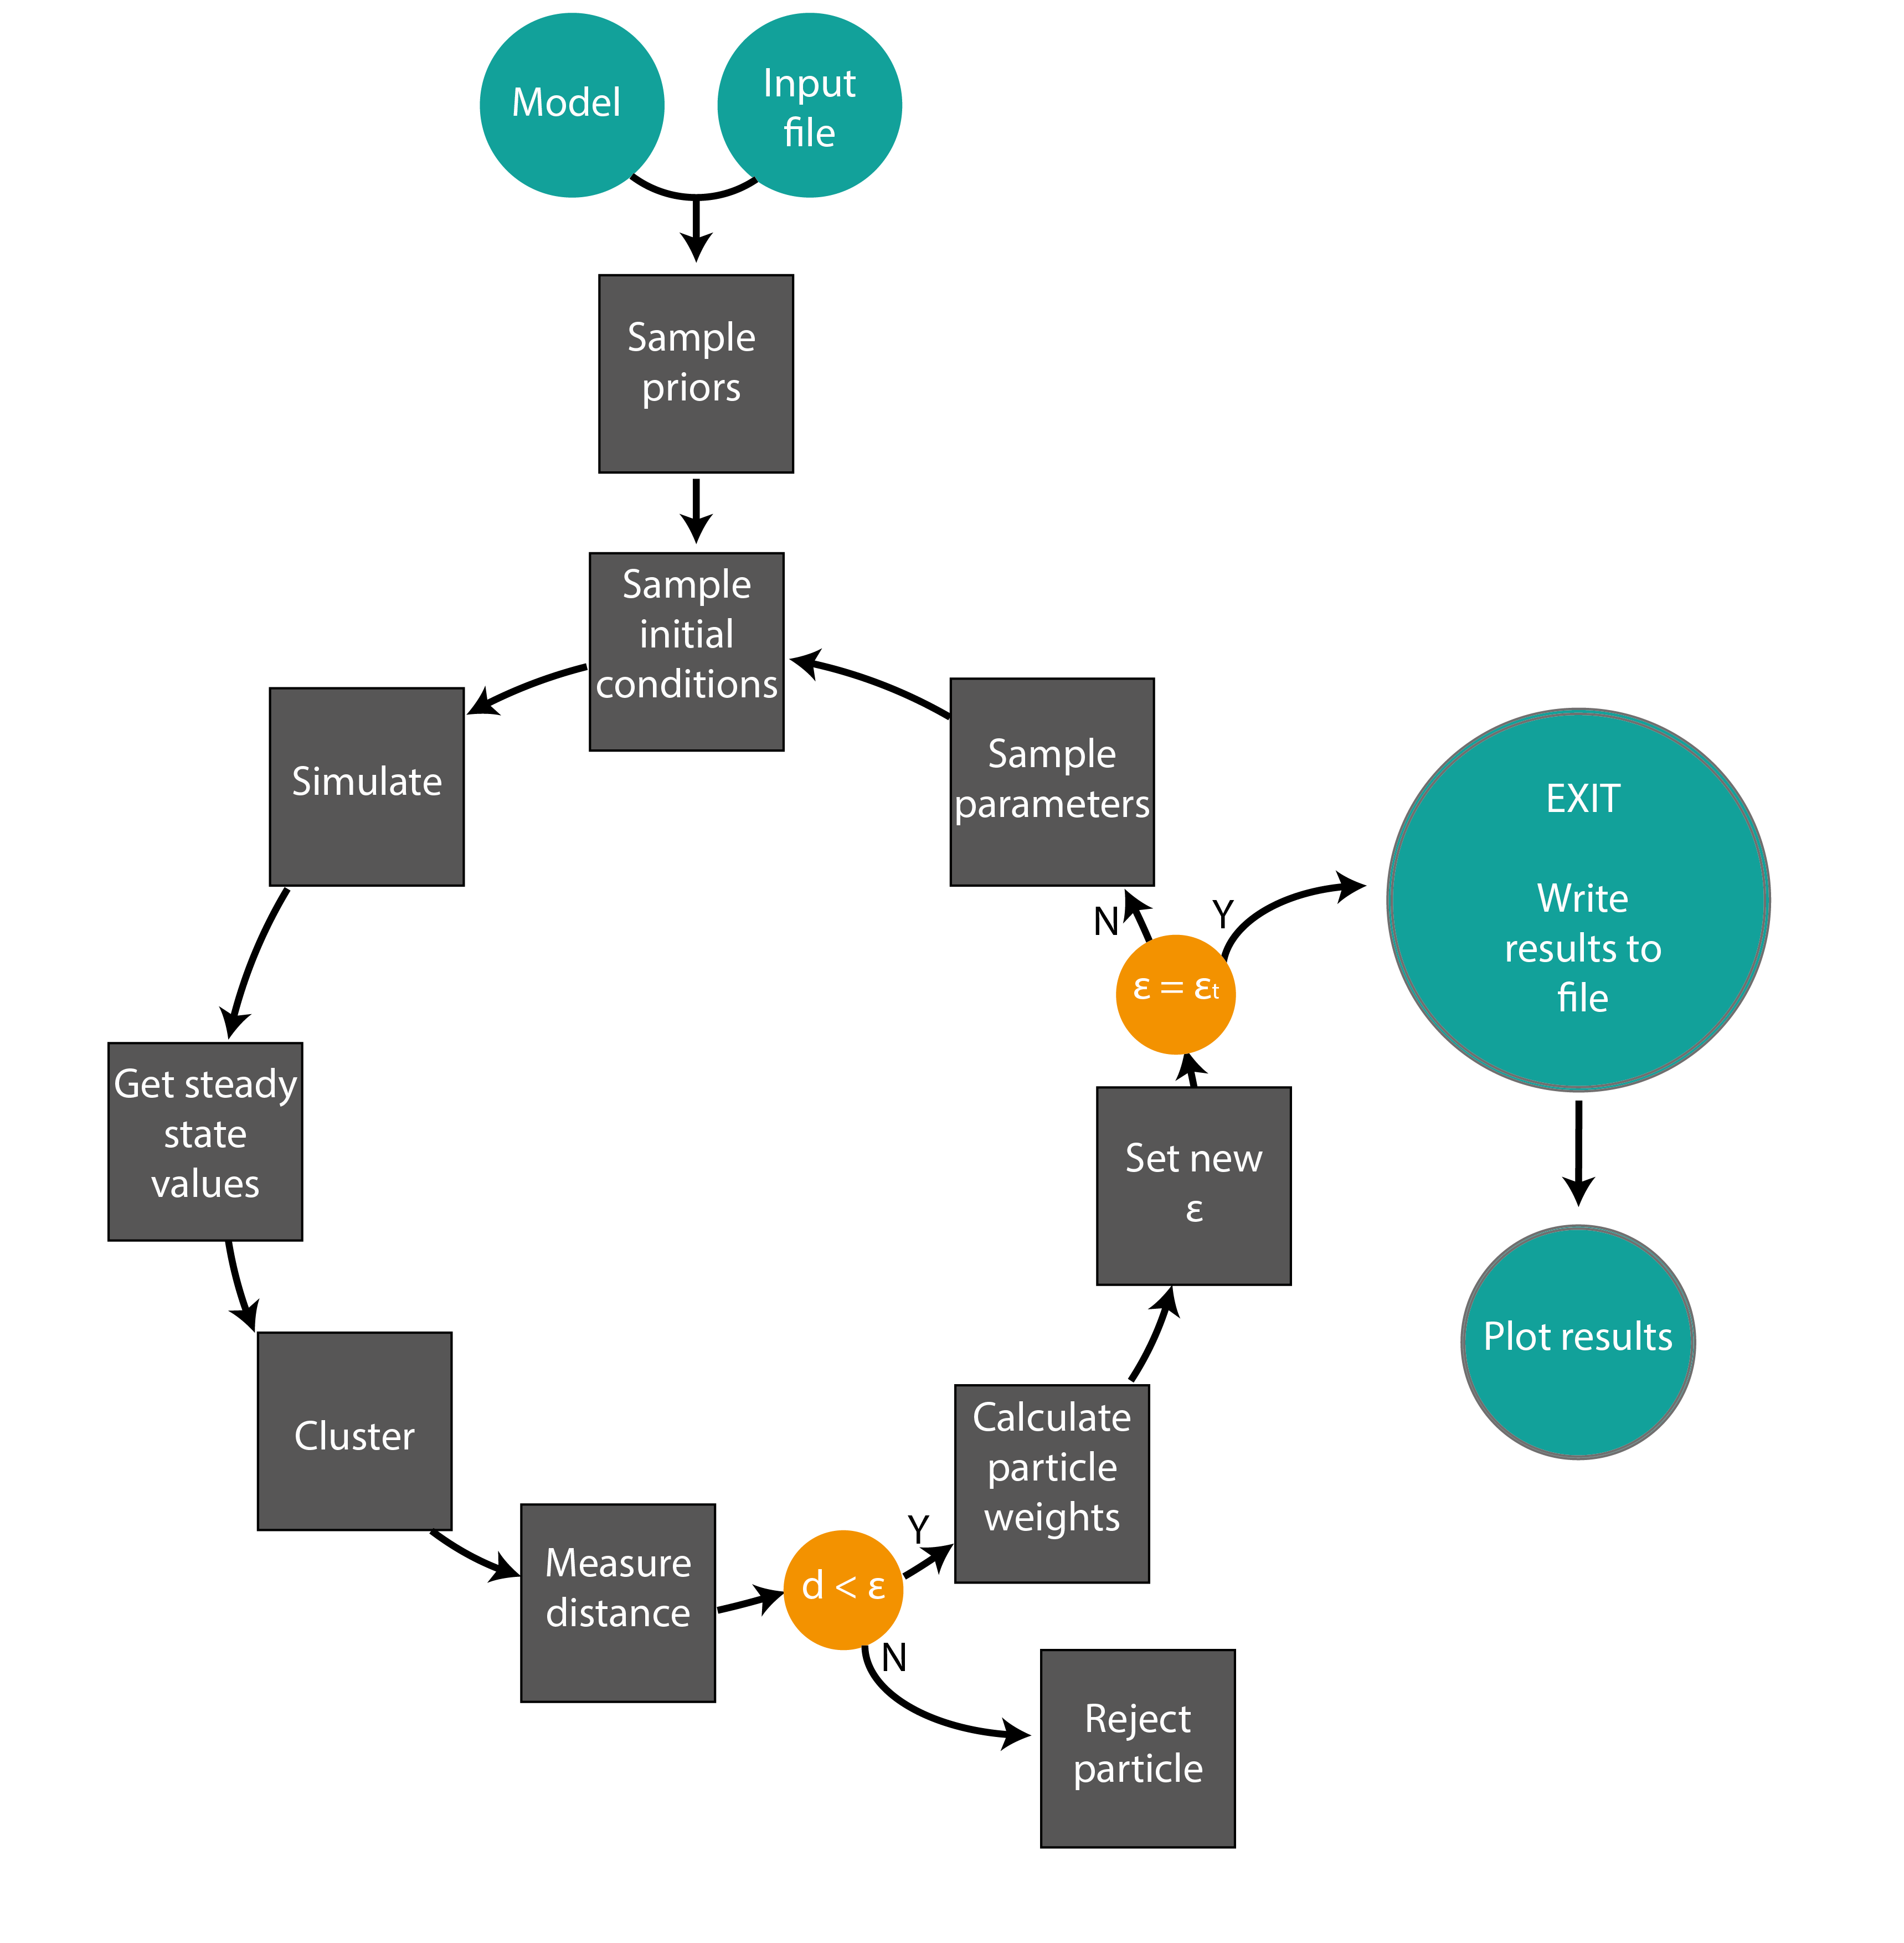
\includegraphics[scale=0.5]{chapterModelling/images/StabilityChecker_flowchart-01}
	\caption[Flowchart of the algorithm used in StabilityChecker]{Flowchart of the algorithm used in StabilityChecker. $\epsilon$ stands for the threshold for the distance from the desired value.}
	\label{fig:flowchart}
\end{figure}

 The user provides the model file, in the form of SBML of cuda as well as the input file. The user input file contains all the necessary information to run the algorithm that is not contained in the model itself. The user specifies the desired stability, the total variance as well as the variance within each cluster that . In addition the user provides the tolerance for the distance from the desired behaviour necessary for the algorithm to terminate. 

 The algorithm begins by sampling from the prior, by selecting a random value from within the user-specified range. Each sample from the priors is called a particle. The number of particles is specified in the user input file. The algorithm then proceeds by sampling initial conditions using Latin Hypercube sampling that ensures an even coverage of values from within the specified range. The model is then simulated for each parameter sample set, for each initial condition set.  It uses cuda-sim software \autocite{Zhou:2011hp} to simulate the models thus taking full advantage of GPUs.  As soon as the simulations are complete, the steady state values for the two species of interest are clustered in order to determine the stability achieved by each parameter sample set. Whether the model has been simulated using ODEs or the Gillespie algorithm dictates the method of clustering used. The two algorithms are summarised in the Appendix. Once the number of clusters present for each parameter set has been determined, the distance from the desired values is measured. If the distance between the simulation and the target behaviour is greater than a predefined threshold distance $\epsilon$, then the parameter values that produced that simulation are rejected. The tolerated distance is first calculated from the samples taken, and then decreased at each iteration until it reaches the final accepted tolerance. This is repeated for a predefined number of samples which are collectively referred to as a population. Each particle in a population has a weight associated with it, which represents the probability of it producing the desired behaviour.At subsequent iterations the new samples are obtained from the previous populations and the $\epsilon$ is set to smaller value, thus eventually reaching the desired behaviour. The algorithm's pseudocode is shown in Algorithm~\ref{alg:StabilityChecker}. 

\begin{algorithm}
	\label{alg:StabilityChecker}
  \caption{StabilityChecker}
 \begin{algorithmic}[1]
    \Statex
	\State Initialise $\epsilon$ 
	\Let{population p}{1}
	\If{p $= 1$}
		\State Sample particles ($\theta$) from priors
		\Else
			\State sample particles from previous population
			\State  Perturb each particle by $\pm$ half the range of the previous population (j) to obtain new perturbed population (i).
	\EndIf
    \State Simulate each particle to obtain steady state values.
    \State Cluster steady state
	\State Reject particles if d $\textgreater$ $\epsilon$.
    \State Calculate weight for each accepted $\theta$
	\State $w_{t}^{(i)} = \begin{cases} 1, & \mbox{if } p = 0 \\\frac{\pi(\theta_{t}^{(i)})}{\sum_{j=1}^N w_{t-1}^{(j)} K_{t}(\theta_{t-1}^{(j)}, \theta_{t}^{(i)})}, & \mbox{if } p \geq  0. \end{cases}$
	\State Normalise weights
	\Repeat {steps 3 - 15} \Until{$\epsilon \leq \epsilon_T$}
  \end{algorithmic}
\end{algorithm}

\subsection{Calculating robustness}

Estimation of system robustness arises naturally from Bayesian methods. By comparing the volume of the posterior to the volume of the prior in a model, one can calculate the robustness of a given model. 
Here we are calculating it using a Monte Carlo sampling accept reject algorithm. Taking a number of random samples from the prior, it keeps track of how many are also found in the posterior. The once that are found in the posterior are accepted and the rest rejected. Robustness is then defined as the number of accepted samples divided by the total number of samples.
\begin{algorithm}
	\label{alg:robustness}
  \caption{Calculating robustness via Monte Carlo sampling rejection }
 \begin{algorithmic}[1]
    \Statex
    \State Sample from priors 
    \State Get min and max boundaries of posterior
	\If{sample within posterior boundaries}
    	\State $accepted += 1$
    \EndIf
    	    	
    \State $acceptance\_rate$ = $\frac{accep
    	ted}{number of samples}$
    \State \Return $acceptance\_rate$
    
  \end{algorithmic}

\end{algorithm}









\section{Results}
\subsection{Testing StabilityChecker: The Gardner toggle switch}

This toggle switch model was developed by T.~S. Gardner~\autocite{Gardner:2000vha}. This model consists of two mutually repressing transcription factors and is defined by the following ODEs:

\begin{align}
\frac{du}{dt} &= \frac{a_1}{1+v^{\beta}} - u \label{eq:gard_1} \\
\frac{dv}{dt} &= \frac{a_2}{1+u^{\gamma }} - v\label{eq:gard_2}
\end{align}
Where $a_1$ and $a_2$ are the effective rates of synthesis of repressors 1 and 2 respectively. \textit{u} is the concentration of repressor 1 and \textit{v} the concentration of repressor 2. \textit{$\beta$} is the cooperativity of repression of promoter 1 and \textit{$\gamma$} of repressor 2. In their paper,  T.~S. Gardner~\autocite{Gardner:2000vha} state that there are two conditions for bistability of this toggle switch model. That $a_1$ and $a_2$ are balanced and that $\beta$ and $\gamma$ are \textgreater 1. In order to test our methodology, we used StabilityChecker to find the posterior distribution for which this model exhibits bistable behaviour. So setting the desired behaviour to bistable, and using for priors a wide range of values that includes the values used in the Gardner paper, we test StabilityChecker to see if it finds the same conditions as the ones set by T.~S. Gardner. The prior distributions used are shown in Table~\ref{tab:gard}. The posterior distribution calculated by StabilityChecker is shown in Figure~\ref{fig:Gard_post}.

\begin{figure}[p]
\centering
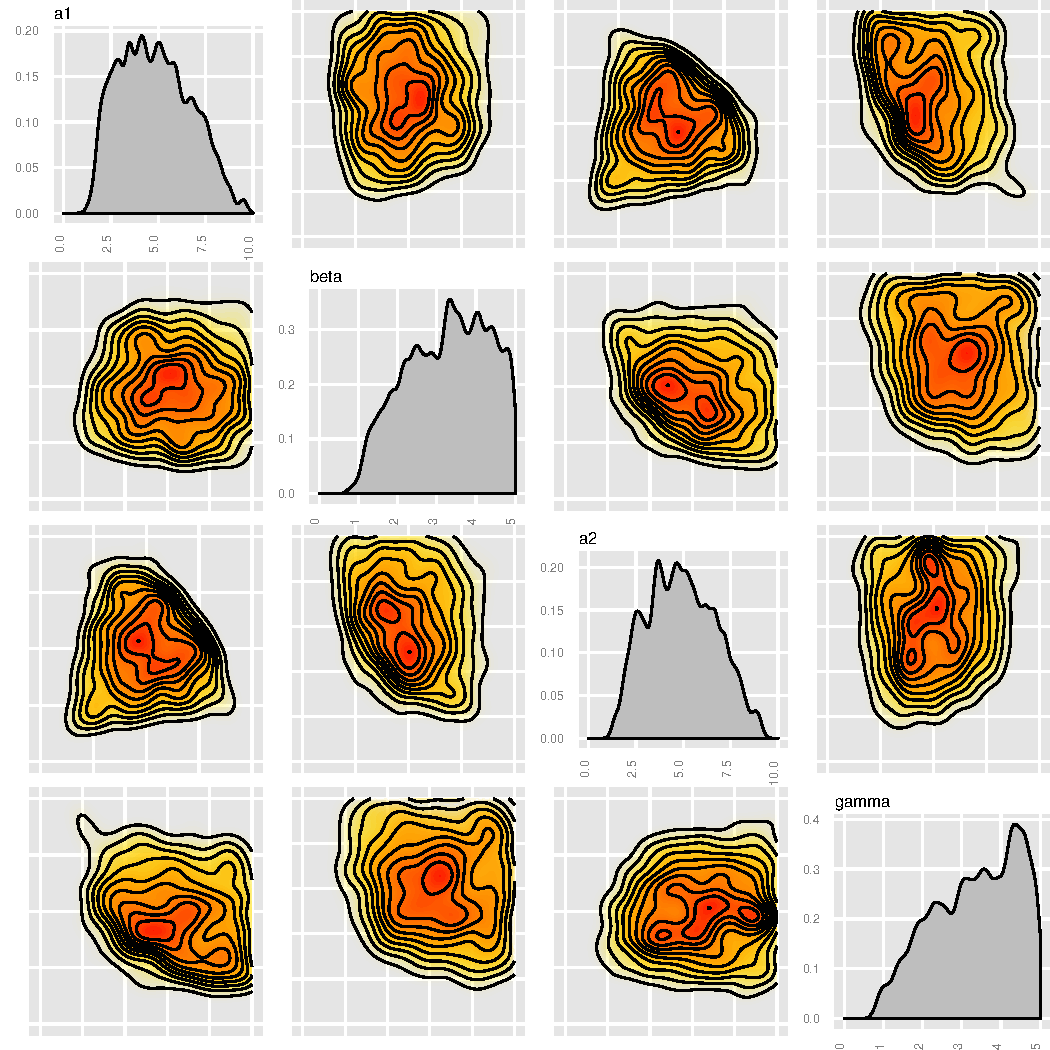
\includegraphics[scale=0.7]{chapterModelling/images/Gardner/posterior.pdf}
\caption[The posterior distribution of the bistable Gardner toggle switch]{The posterior distribution of the bistable Gardner toggle switch. The parameters $a_1$, $a_2$ represent to the effective synthesis rate of repressors 1 and 2 respectively. Parameters $\beta$, $\gamma$ represent the cooperativity on repressors 1 and 2 respectively. The marginal distributions of each parameter are found on the diagonal and pairwise joint distributions along the sides.}
\label{fig:Gard_post}
\end{figure}

\clearpage
\begin{figure}[p]
\centering
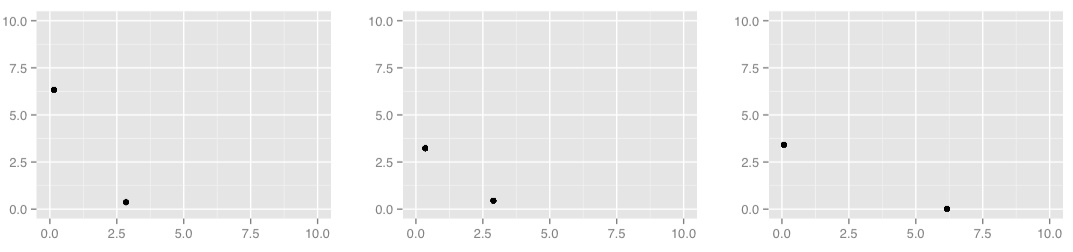
\includegraphics[scale=0.4]{chapterModelling/images/Gardner/phase_plots.png}
\caption{A sample of the phase plots produced from the final population of the Gardner switch.}
\label{fig:det_gard_phase}
\end{figure}

\begin{table}[p]
\centering
\caption{Gardner switch priors}
\label{tab:gard}
\begin{tabular}{cccc|cc}
\multicolumn{4}{c|}{Parameters} & \multicolumn{2}{c}{Species} \\ %\hline
$a_1$   & $\beta$   & $a_2$   & $\gamma$  &   $s_1$      &       $s_2$   \\
0-10    & 0-5       & 0-10    &  0-5      &      0-100   &          0-100   
\end{tabular}
\end{table}

These results agree with the results reported by the original paper~\autocite{Gardner:2000vha} . For this switch to be bistable $a_1$ and $a_2$ must be balanced while $\beta$ and $\gamma$ must both be \textgreater 1, as can be seen in the marginal distributions of $\beta$ and $\gamma$ in Figure~\ref{fig:Gard_post}. The conditions set by the original paper for parameters $a_1$ and $a_2$ are met, as the joint distribution shown in Figure~\ref{fig:Gard_post} matches the bifurcation lines calculated in the original paper. 
This successful test demonstrates that StabilityChecker can be used to find the stability a model is capable of as well as the parameter ranges that can produce that. This allows us to confidently apply the methodology to further models.
%-%-%-%-%-%-%%-%-%-%-%-%-%%-%-%-%-%-%-%
\newpage
\subsubsection{Comparing the deterministic and stochastic cases} 
    
There are two main ways of modelling a system, deterministically and stochastically. Deterministic modelling utilises ordinary differential equations (ODE) and models the concentrations of the species (proteins or other molecules) by time-dependent variables~\autocite{deJong:2002ft}. Rate equations are used to model gene regulation where the rate of production of a species is a function of the concentrations of the other species~\autocite{deJong:2002ft}. When modelling deterministically the model is viewed as a system which, with sufficient knowledge of the system, its behaviour is entirely predictable. Nevertheless we are still a long way away from having complete knowledge of a system of interesting size~\autocite{wilkinson:2006}. Deterministic modelling also assumes a homogenous mixture where species concentrations vary continuously and deterministically, assumptions that often are not met \textit{in vivo}. A cell is spatially and temporally separated, due to small molecule numbers and fluctuations in the timing of processes~\autocite{deJong:2002ft}.  
   
In stochastic modelling, species are measured in discrete amounts rather than concentrations and a joint probability distribution is used to express the probability that at time \textit{t} the cell contains a number of molecules of each species~\autocite{deJong:2002ft}. It takes uncertainty into account and does not assume a homogenous mix. It is thus often more appropriate for modelling cellular systems, although more computationally intensive. In stochastic systems the Gillespie algorithm is widely used to simulate the time-evolution of the state of the system~\autocite{Warren:2005kea}.

The toggle switch has been modelled both deterministically and stochastically, with the two methods producing different results. Thus here we use StabilityChecker to compare the stabilities that the model is capable of, under the different simulation types. By using the same framework, and the same prior distributions for the models, one can directly compare the posterior distributions produced by the deterministic and the stochastic case, and uncover the effects that are due to the stochasticity of the system. This is relevant in a a biological model in which small molecule numbers and external noise are not negligible. Using StabilityChecker and using the same priors for the two models (Table~\ref{tab:gard_det_stoch}), we calculated the posterior for each both bistable models. The results are shown in Figures~\ref{fig:Gard_post_det_high},~\ref{fig:Gard_post_stch}. The prior ranges used are much wider than in the test case in order to allow more flexibility in both models and have a greater range over which to compare the models. 

\clearpage
\begin{table}[p]
\centering
\caption{Gardner switch priors}
\label{tab:gard_det_stoch}
\begin{tabular}{cccc|cc}
\multicolumn{4}{c|}{Parameters} & \multicolumn{2}{c}{Species} \\ %\hline
$a_1$   & $\beta$   & $a_2$   & $\gamma$  &   $s_1$      &       $s_2$   \\
0-60    & 0-5       & 0-60    &  0-5      &      0-100   &          0-100   
\end{tabular}
\end{table}


\begin{figure}[p]
\centering
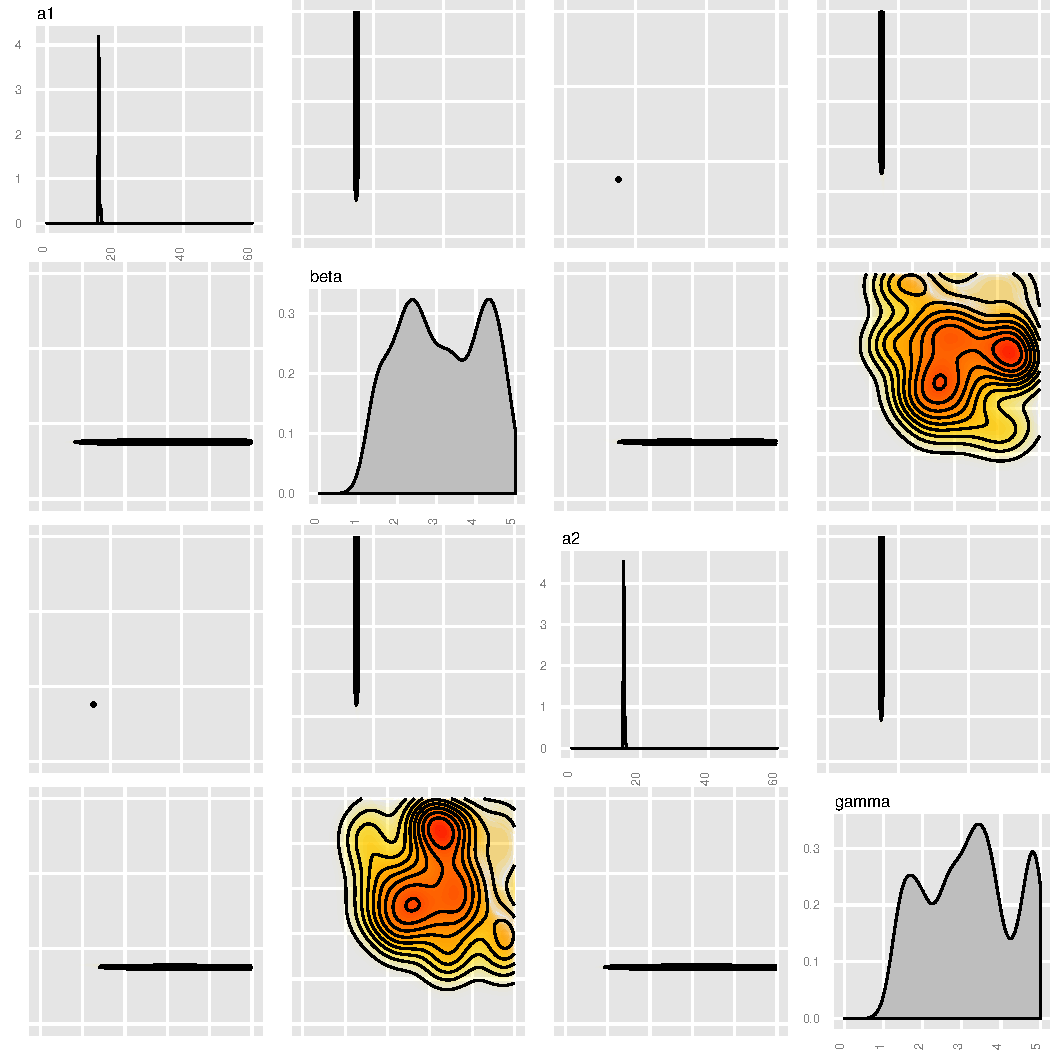
\includegraphics[scale=0.7 ]{chapterModelling/images/Gardner/posterior_det_high_mean.pdf}
\caption{The posterior distribution of the deterministic model of the Gardner toggle switch.}
\label{fig:Gard_post_det_high}
\end{figure}
\newpage

\begin{figure}[p]
\centering
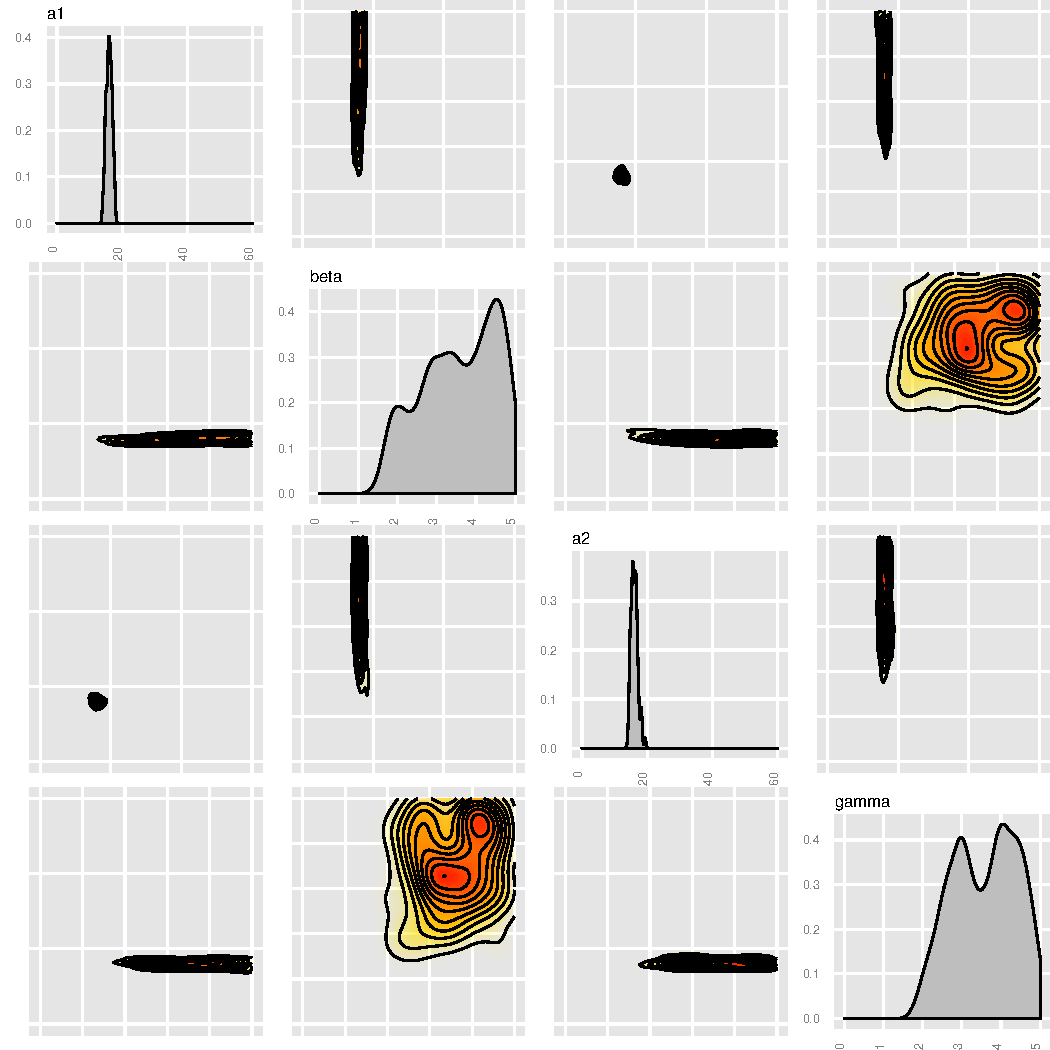
\includegraphics[scale=0.7]{chapterModelling/images/Gardner/posterior_stch_high_mean.pdf}
\caption{The posterior distribution of the stochastic model of the Gardner toggle switch.}
\label{fig:Gard_post_stch}
\end{figure}

As can be seen in the above results, stochasticity has a big effect on the posterior. Firstly, a greater parameter range can produce a bistable behaviour when stochastic effects are taken into account. The condition set by T.~S Gardner~\autocite{Gardner:2000vha} for the values of $a_1$ and $a_2$ to be balanced holds in both the deterministic and stochastic cases but in the stochastic case this is met by a wider range of values. The second conditions of $\beta$  and $\gamma$ \textgreater 1 also needs to be met in the stochastic case. 

\begin{figure}[p]
\centering
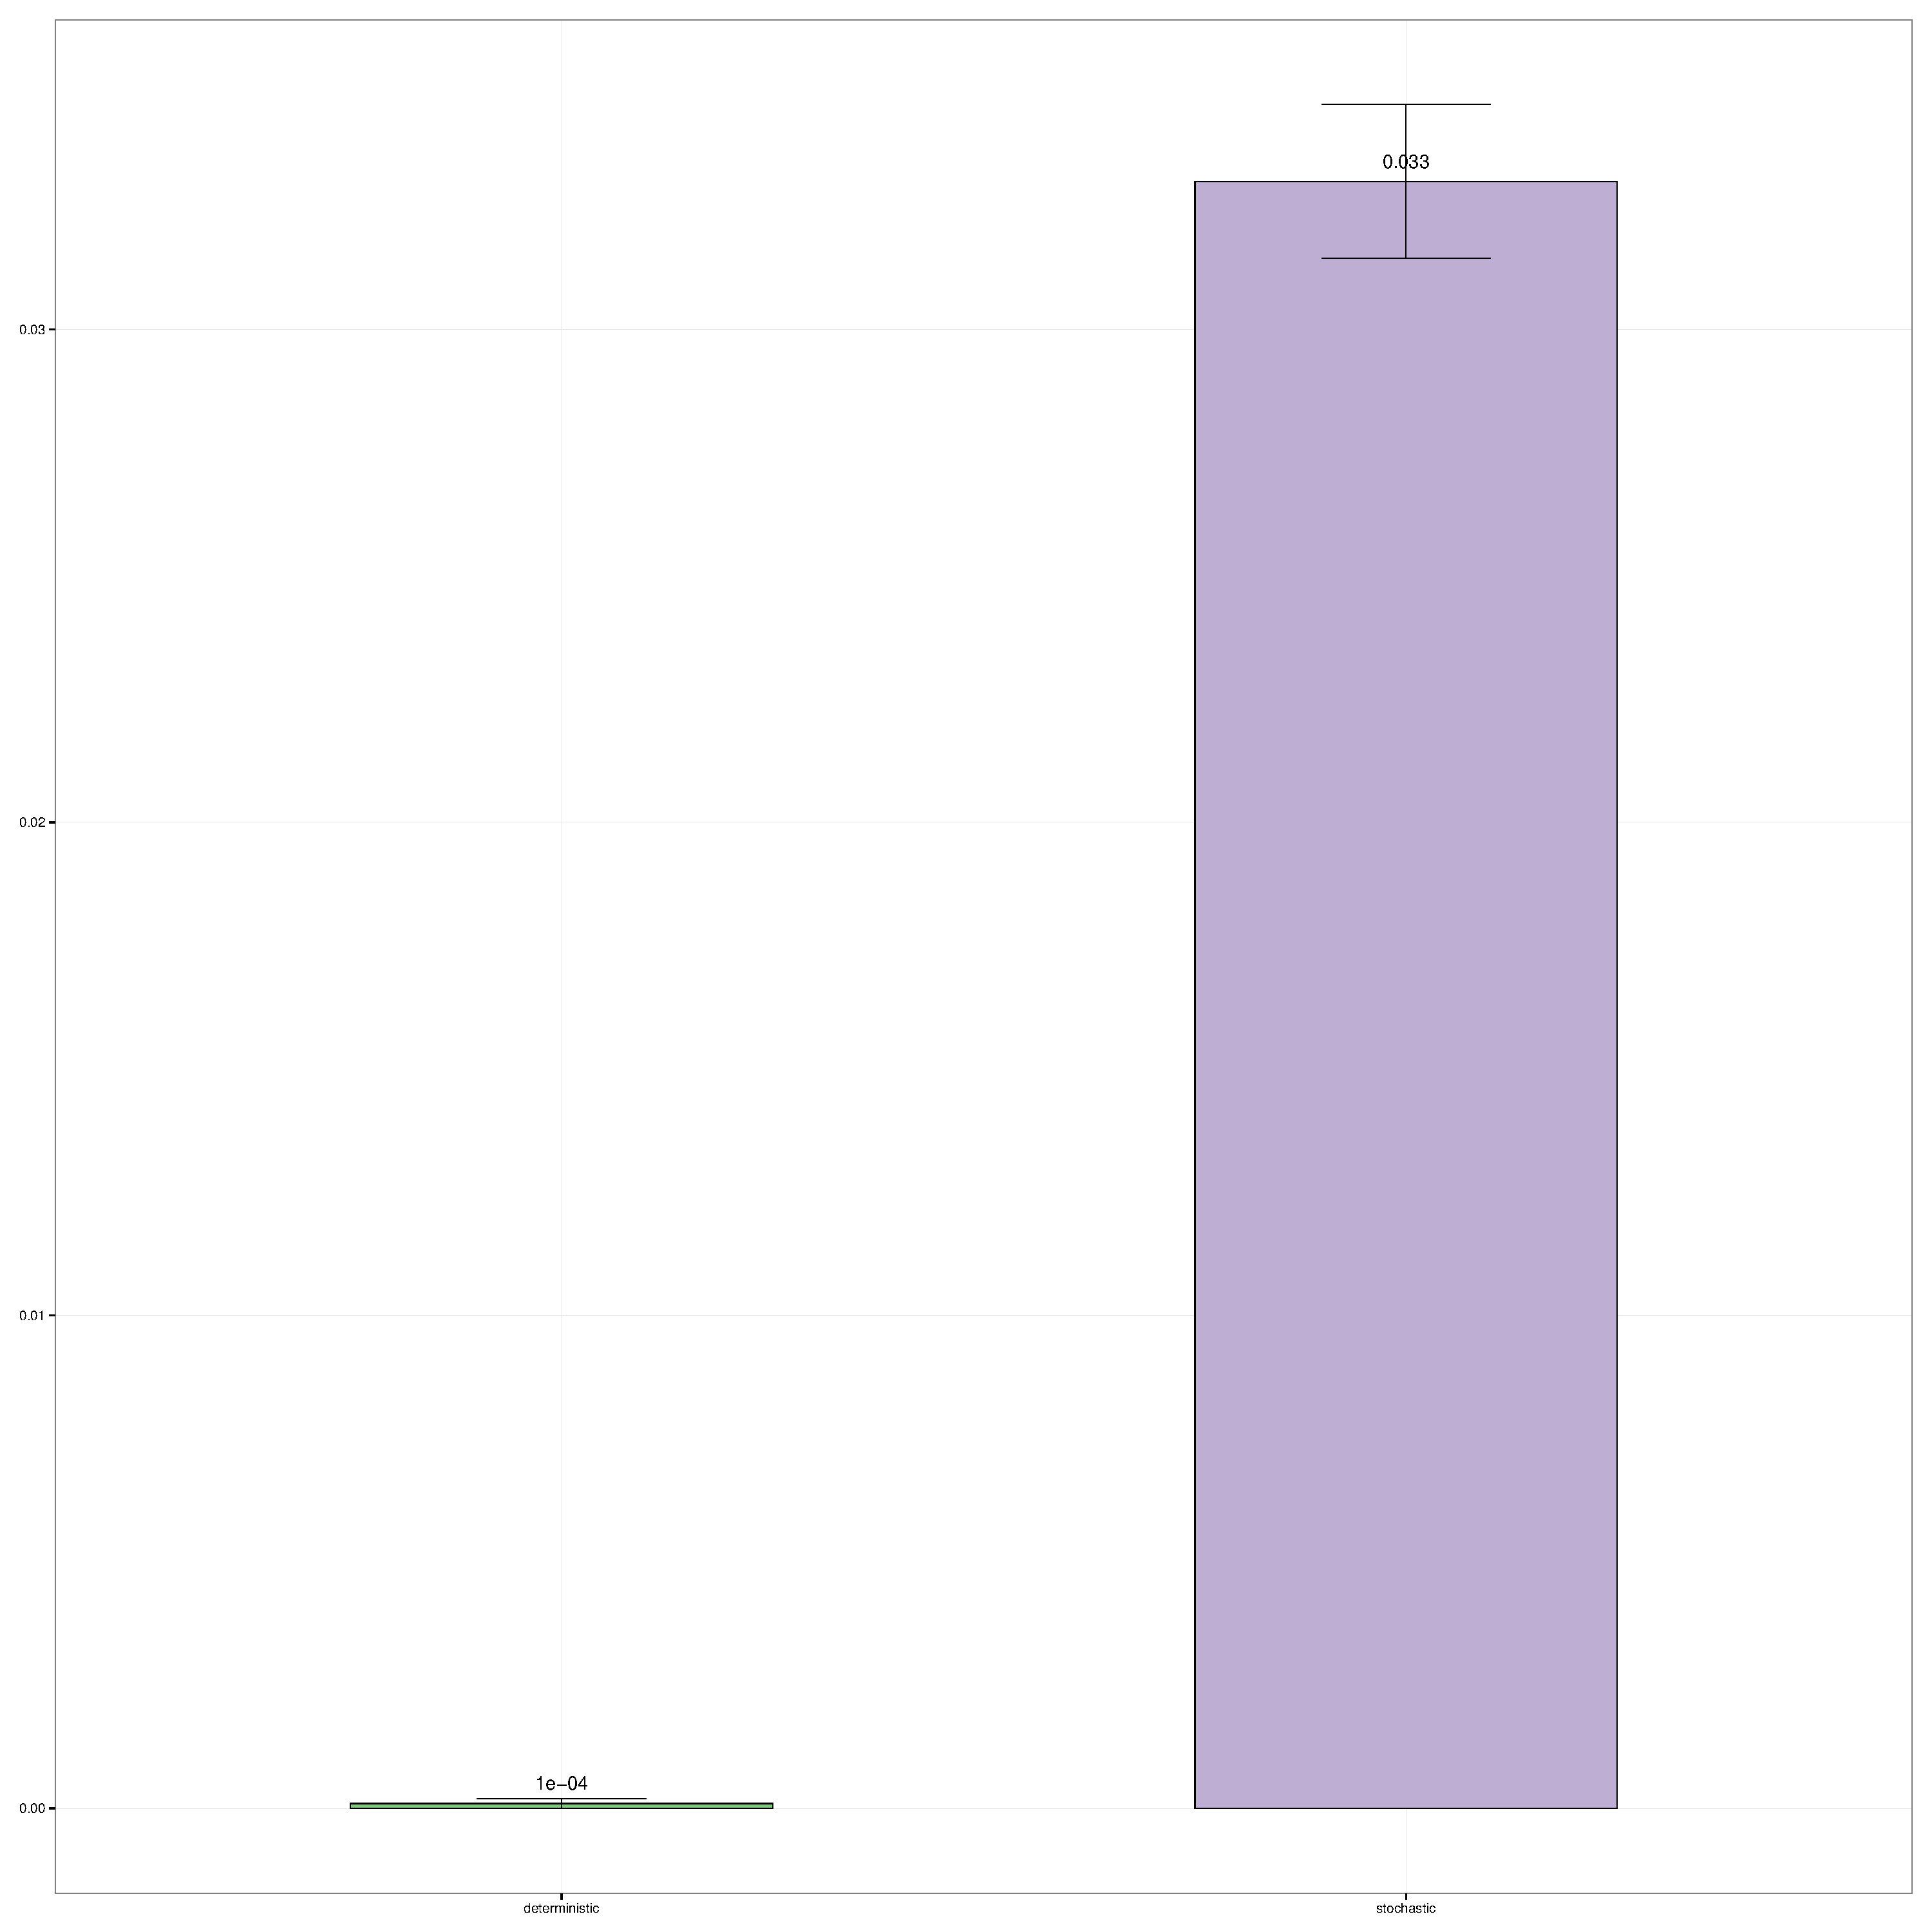
\includegraphics[scale=0.2]{chapterModelling/images/Gardner/robustness_comparison_high_mean.pdf}
\caption{Comparing the robustness of the deterministic and stochastic Gardner switch models}
\label{fig:Gard_robst}
\end{figure}

 When stochasticity is taken into account, robustness increases significantly as seen in Figure~\ref{fig:Gard_robst}. This indicates that stochasticity increases the ability of the model to withstand fluctuations in parameter values and still produce the desired bistability. A deterministic model cannot predict this increased robustness.


%-%-%-%-%-%-%-%-%-%-%-%-%-%-%-%-%-%-%-%-%-%-%-%-%-%-%-%-%-%-%-%-%-%-%-%-%-%-%-%-%-%-%-%-%-%-%-%-%-%
\newpage
\section{Lu toggle switch models}

In their study, \textcite{Lu:2013br} explored the effect of white Gaussian and shot noise on the multi-state switches. They found that the classical toggle switch, with the repressing transcription factors has two steady states and the toggle switch with added double positive auto-regulation has three steady states. By extending the analysis on these models by using StabilityChecker we can determine the design principles that make a tristable versus a bistable switch. This is another example of a use for StabilityChecker.
The system used in their study is defined by two dynamical systems:

\begin{align}
\dot{x} &= f_{x}(x,y) =g_{x}\, H^{S}_{xy}(y)\, H^{S}_{xx}\,(x)-k_{x}x \label{eq:lu_both_1} \\
\dot{y} &= f_{y}(x,y) =g_{y}\,H^{S}_{yx}(x)\,H^{S}_{yy}\,(y)-k_{y}y \label{eq:lu_both_2}
\end{align}
\begin{align}
H^{S}_{xx} &= H^{-}_{x}(x)+\lambda_{x}H^{+}_{x}(x)\label{eq:lu_hsxx}\\
H^{-}_{x}(x) &= 1 \big/\left[1+(x/a_{x})^{n_{x}}\right]\label{eq:lu_hpx}\\
H^{+}_{x}(x) &= 1-H^{-}_{x}(x)\label{eq:lu_hmx}
\end{align}
%\begin{align*}%
%	\left\{S^3_\text{this} \frac{1}{2}\right.
%\end{align*}

For the classical model, in which no self-activation is present, the system reduces to the following equations:

\begin{align}
\dot{x}=f_{x}(x,y) &= g_{x}H^{S}_{xy}(y)-k_{x}x,\label{eq:lu_cl_1}\\
\dot{y}=f_{y}(x,y) &= g_{y}H^{S}_{yx}(x)-k_{y}y\label{eq:lu_cl_2}
\end{align}
For the parameter values used in the Lu study, as shown in Table ~\ref{tab:lu_cl_bi}, the system exhibits three positive steady states (Figure ~\ref{fig:lu_bis_class}), of which two are stable and one is unstable. 

\clearpage
\begin{figure}[p]
\centering
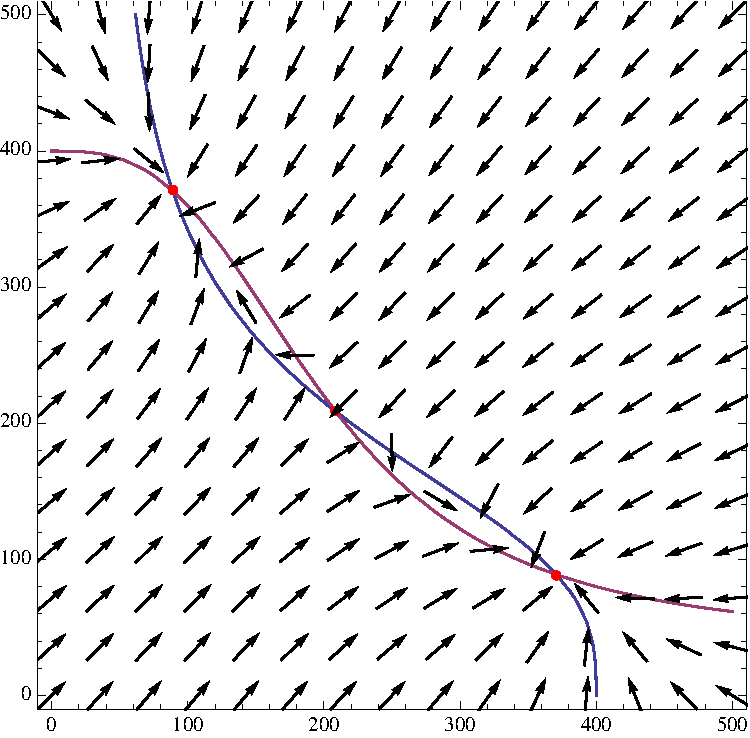
\includegraphics[scale=0.7]{chapterModelling/images/Lu/mae/classic.pdf}
\caption[Phase portrait of the Lu classical model with no self activation]{Phase portrait of the Lu classical model with no self activation. There are two stable steady states and one unstable steady state.}
\label{fig:lu_bis_class}
\end{figure}

\begin{table}[p]
\centering
\caption{Lu classical model parameter values}
\label{tab:lu_cl_bi}
\begin{tabular}{cccccccccc}
gx    & gy    & kx    & ky    & nxy & nyx & xxy     & xyx     & Ixy   & Iyx \\
40&40     &0.1   & 0.1   &  3  &  3  &  200    &  200    & 0.1    &   0.1
\end{tabular}
\end{table}

Using StabilityChecker with priors centred around the parameter values used in the original paper (Table ~\ref{tab:lu}), we can find the robustness of this bistable behaviour, as well as identify the most important parameters for bistability. The posterior distribution of this model is shown in Figure ~\ref{fig:lu_bistable}. As can be seen from the posterior, the most restrained parameters are kx and ky, the parameters responsible for the degradation of the species involved. This indicates that the rate of degradation of the species is critical for the desired dynamic to occur. 

\begin{figure}[p]
\centering
\includegraphics[scale=0.8]{chapterModelling/images/Lu/posterior_100p_narrow.pdf}
\caption[The posterior distribution of the Lu classical model with no self activation]{The posterior distribution of the Lu classical model with no self activation. kx and ky are the most constrained parameters.}
\label{fig:lu_bistable}
\end{figure}


\clearpage
\begin{figure}[p]
\centering
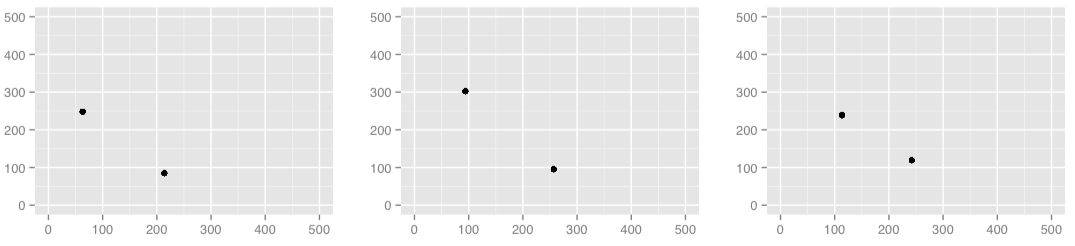
\includegraphics[scale=0.4]{chapterModelling/images/Lu/phase_plot.png}
\caption{A sample of the phase plots produced from the final population of the Lu classical model.}
\label{fig:lu_phase}
\end{figure}

\begin{table}[p]
\centering
\caption{Lu classical model priors}
\label{tab:lu}
\begin{tabular}{cccccccccc}
gx    & gy    & kx    & ky    & nxy & nyx & xxy     & xyx     & Ixy   & Iyx \\
35-45 & 35-45 & 0-0.2 & 0-0.2 & 2-4 & 2-4 & 150-250 & 150-250 & 0-0.2 &   0-0.2 
\end{tabular}
\end{table}

If self-activation is included, then the system is that presented in equations \eqref{eq:lu_both_1, eq:lu_both_2} . When values that are presented in table 1 are assigned to the parameters for the self-activating model, the system exhibits five positive steady states~\ref{fig:lu_tri_phse}. 

\clearpage
\begin{table}[p]
\centering
\caption{Lu model with self-activation parameter values}
\label{tab:lu_dp_tri}
\begin{tabular}{cccccccccc}
gx    & gy    & kx    & ky    & nxy & nyx & xxy     & xyx     & Ixy   & Iyx \\
4&4     &0.1   & 0.1   &  1  &  1  &  200    &  200    & 0.1    &   0.1
\end{tabular}
\end{table}

\begin{figure}[p]
\centering
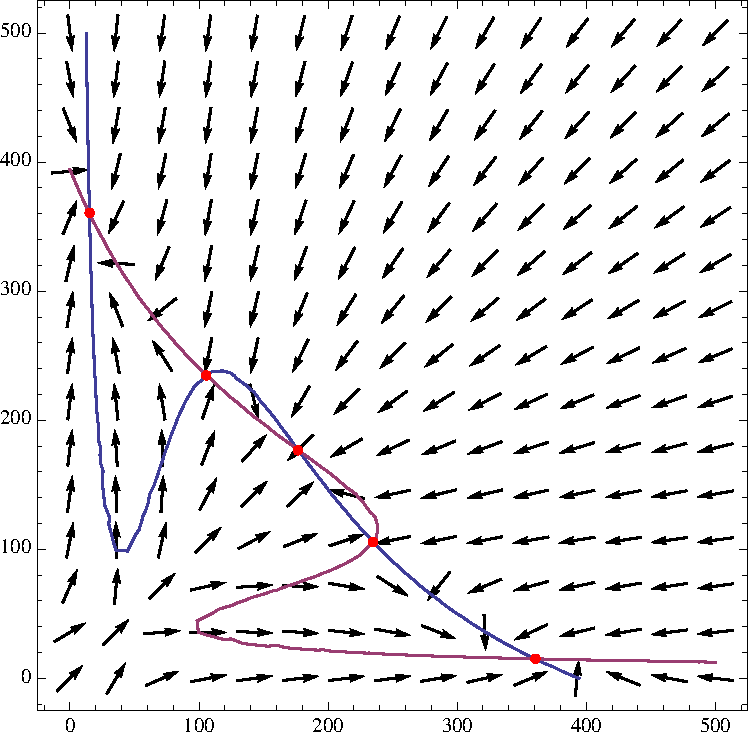
\includegraphics[scale=0.7]{chapterModelling/images/Lu/mae/selfactivation.pdf}
\caption[Phase portrait of the Lu model including double self-activation]{Phase portrait of the Lu model including double self-activation. The model had three stable steady states and two unstable steady states.}
\label{fig:lu_tri_phse}
\end{figure}

Using StabilityChecker and priors centred around the original values, shown in Table~\ref{tab:lu_dp_pr}, we can explore the robustness of this behaviour, in a similar way as done for the classical model. The posterior is shown in Figure~\ref{fig:lu_tristable}. The most constrained parameters are kx and ky, similar as in the classic toggle switch case.

\clearpage
\begin{table}[p]
\centering
\caption{Lu model with double self-activation priors}
\label{tab:lu_dp_pr}
\begin{tabular}{cccccccccc}
gx    & gy    & kx    & ky    & nxy & nyx & xxy     & xyx     & Ixy   & Iyx \\
3-5 & 3-5 & 0-0.2 & 0-0.2 & 0-2 & 0-2 & 150-250 & 150-250 & 0-0.2 &   0-0.2 
\end{tabular}
\end{table}

\begin{figure}[p]
\centering
\includegraphics[scale=0.3]{chapterModelling/images/Lu/tri/posterior_1000p_1.pdf}
\caption[The posterior distribution of the Lu model with double self activation]{The posterior distribution of the Lu model with double self activation. kx and ky are the most constrained parameters.}
\label{fig:lu_tristable}
\end{figure}


\begin{figure}[p]
\centering
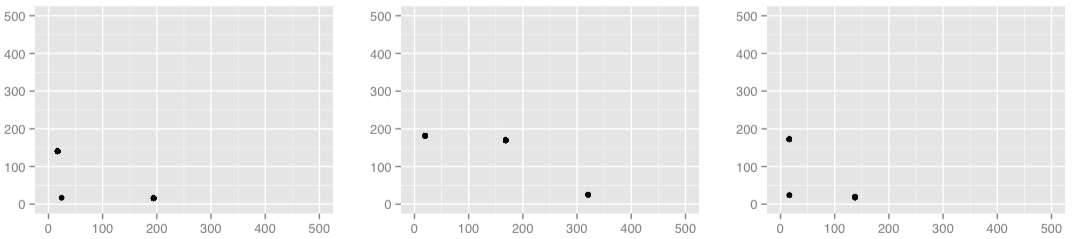
\includegraphics[scale=0.4]{chapterModelling/images/Lu/tri/phase_plots.png}
\caption{A sample of the phase plots produced from the final population of the Lu tristable model.}
\label{fig:lu_tri_phase_pl}
\end{figure}


\subsubsection{Extracting switch design principles}
Next, we went on to study the design principles that make a switch tristable vs bistable. To do this we implemented an algorithm, as shown in the Appendix. Samples were taken from posterior distribution of the Lu tristable switch. Then we separate the values, for each parameter, that were also found in the posterior of the bistable switch. The same procedure was done but taking samples from the bistable posterior and looking for them in the tristable posterior. This can give an indication of the separation of parameter values that can give rise to a bistable vs a tristable switch. 

The results are shown in Figure ~\ref{fig:lu_bi_tri}.
\clearpage
\begin{figure}[p]
\centering
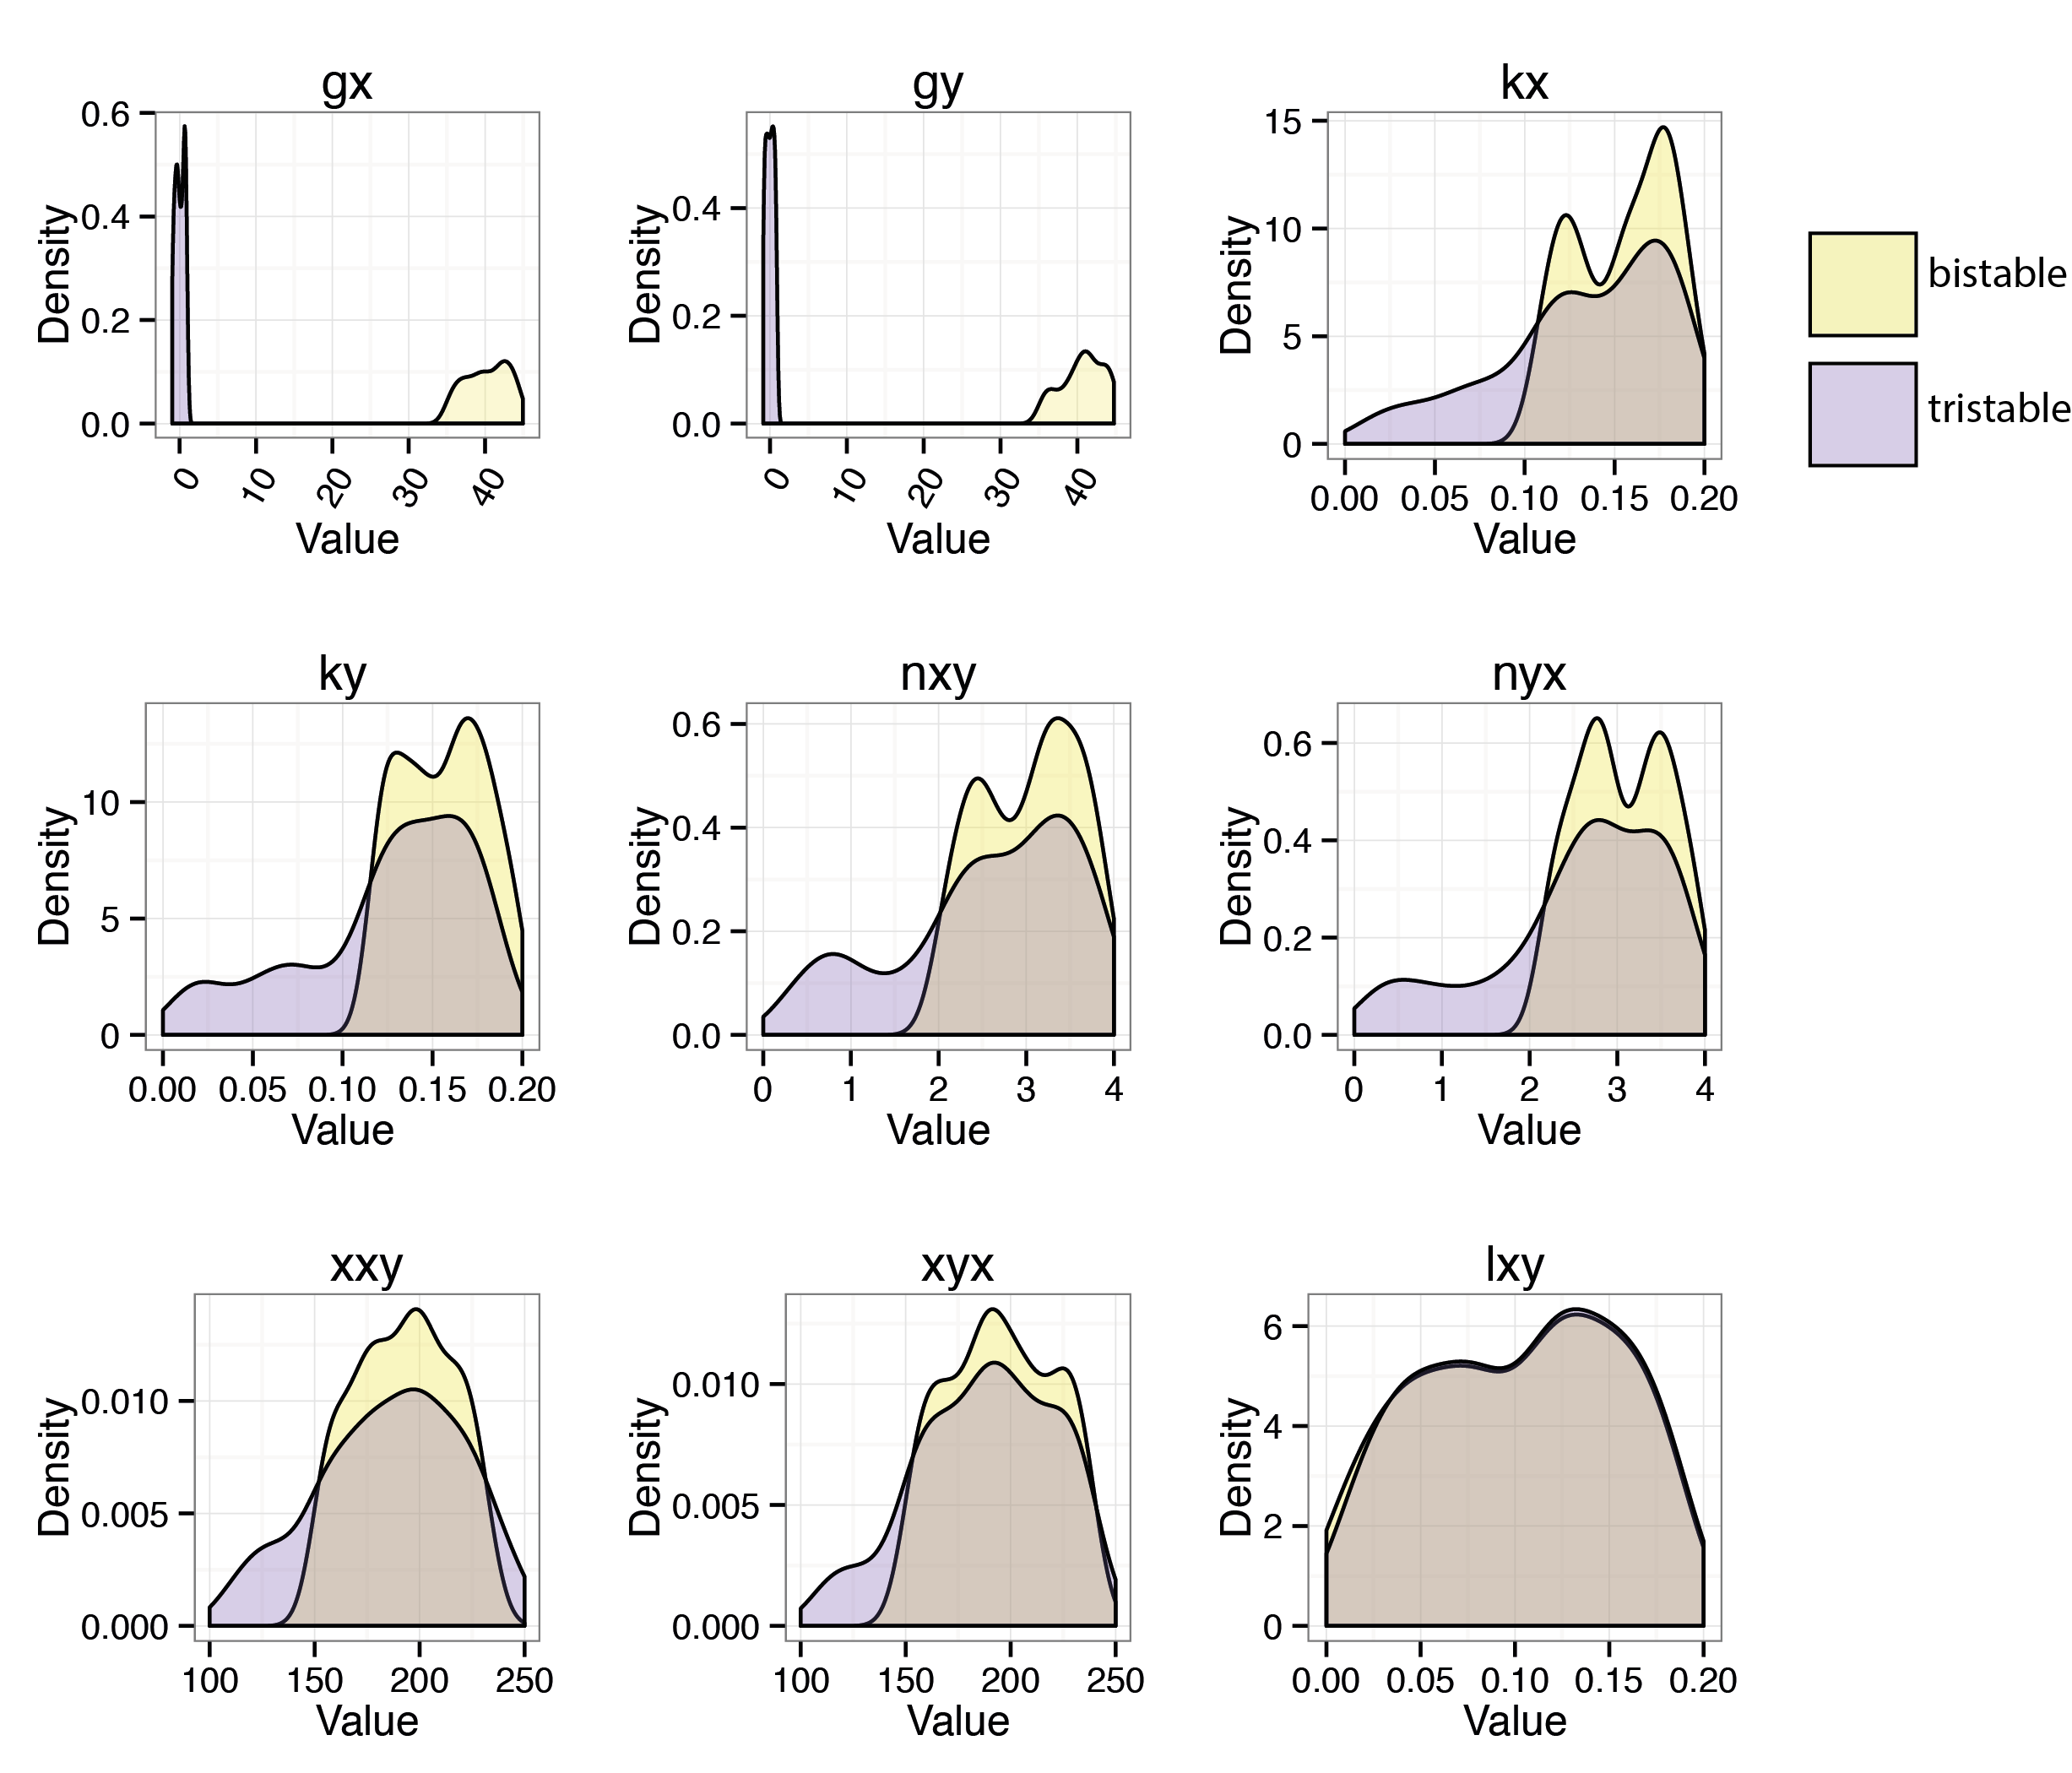
\includegraphics[scale=0.8]{chapterModelling/images/design_principles/res_all_tri_biyp.png}
\caption{Extracting the tristable versus bistable switch design principles}
\label{fig:lu_bi_tri}
\end{figure}

It is clear from the above results that the values for gx and gy are very different for producing a bistable versus a tristable switch. In order to further test this result, we used the model with self activation, with the same priors as used in the tristable case (Table~\ref{tab:lu_dp_tri}), except for the values of gx and gy, which we swapped for the values found to produce a bistable switch. This new model was then analysed using StabilityChecker and was found to be bistable. This indicates that the values of gx and gy, representing gene expression, are critical for the design of a switch with a given stability, and changing their values can make a tristable switch bistable. This can be seen in the phase plots produced, shown in Figure~\ref{fig:lu_bi_tri}

\begin{figure}[p]
\centering
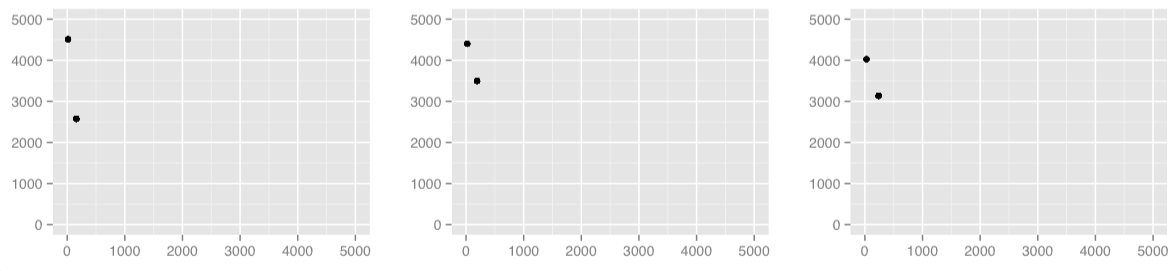
\includegraphics[scale=0.4]{chapterModelling/images/Lu/tri/phase_plot_tri_bi.png}
\caption{The phase plots produced by the last population of StabilityChecker. By changing only the parameters gx and gy in the Lu model with self-activation, the switch became a bistable switch, instead of a tristable switch.}
\label{fig:lu_bi_tri}
\end{figure}


%-%-%-%-%-%-%-%-%-%-%-%-%-%-%-%-%-%-%-%-%-%-%-%-%-%-%-%-%-%-%-%-%-%-%-%-%-%-%-%-%-%-%-%-%-%-%-%-%-%
\newpage
\subsection{Positive auto-regulation increases robustness to parameter fluctuations}

When faced with a set of competing designs for a given genetic circuit, one is likely to choose the simplest possible model that can achieve the desired behaviour. However, simple systems are often the least robust. Feedback loops are well known key regulatory motifs \autocite{Brandman:2005ci}. Negative feedback loops are essential for homeostasis and buffering \autocite{Thomas:1995id} thus increasing robustness to extrinsic noise sources and positive feedback loops can generate multistationarity in a system \autocite{Thomas:1995id}. Incorporating this kind of additional feedback interactions can make a design more robust and reliable. 

Building robust devices is critical for the success of synthetic biology. A robust device is a device that can withstand fluctuations in parameter values and still produce the desired behaviour. Here we use StabilityChecker to compare the robustness of two switches, a simple toggle switch and a switch with added positive auto-regulation. These models avoid the quasi-steady state approximation (QSSA) often used in modelling the toggle switch. Since StabilityChekcker is able to analyse models with numerous equations and parameters, there is no need for this assumption, which approximates a solution. Using Mass Action, the two models used are shown below:

Standard toggle switch:
$$
\begin{array}{cccc}
      \textrm{gA}\stackrel{\textrm{ge}}{\longrightarrow}\textrm{gA} + \textrm{A} \\
      \textrm{gB}\stackrel{\textrm{ge}}{\longrightarrow}\textrm{gB} + \textrm{B} \\
      \textrm{A} + \textrm{A} \stackrel{\textrm{dim}}{\longrightarrow}\textrm{A2} \\
      \textrm{A2} \stackrel{\textrm{dim r}}{\longrightarrow}\textrm{A} + \textrm{A} \\
      \textrm{B} + \textrm{B} \stackrel{\textrm{dim}}{\longrightarrow} \textrm{B2} \\
      \textrm{B2} \stackrel{\textrm{dim\_r}}{\longrightarrow}\textrm{B} + \textrm{B} \\
      \textrm{gA} + \textrm{B2} \stackrel{\textrm{rep}}{\longrightarrow}\textrm{B2gA} \\
      \textrm{B2gA} \stackrel{\textrm{rep\_r}}{\longrightarrow}\textrm{B} + \textrm{gA} \\
      \textrm{gB} + \textrm{A2} \stackrel{\textrm{rep}}{\longrightarrow}\textrm{A2gB} \\
      \textrm{A2gB} \stackrel{\textrm{rep\_r}}{\longrightarrow}\textrm{A2} + \textrm{gB} \\
      \textrm{A} \stackrel{\textrm{deg}}{\longrightarrow}\textrm{\O}\\
      \textrm{B} \stackrel{\textrm{deg}}{\longrightarrow}\textrm{\O}\\
      \textrm{S} + \textrm{A2} \stackrel{\textrm{rep\_dim}}{\longrightarrow}\textrm{SA2}\\
      \textrm{SA2} \stackrel{\textrm{rep\_dim\_r}}{\longrightarrow}\textrm{S} + \textrm{A2}\\
      \textrm{R} + \textrm{B2} \stackrel{\textrm{rep\_dim}}{\longrightarrow}\textrm{RB2}\\
      \textrm{RB2} \stackrel{\textrm{rep\_dim\_r}}{\longrightarrow}\textrm{R} + \textrm{B2}\\
      \textrm{R} \stackrel{\textrm{deg}}{\longrightarrow} \textrm{\O}\\
      \textrm{S} \stackrel{\textrm{deg}}{\longrightarrow}\textrm{\O}\\
\end{array}
$$

Double positive autoregulation:
$$
\begin{array}{cccc} 
    \textrm{A2} + \textrm{gA} \stackrel{\textrm{aut 1}}{\longrightarrow} \textrm{A2gA} \\
    \textrm{A2gA} \stackrel{\textrm{aut 2}}{\longrightarrow} \textrm{A} + \textrm{A2gA}\\
    \textrm{A2gA} \stackrel{\textrm{aut 3}}{\longrightarrow} \textrm{A2}+ \textrm{gA}  \\
    \textrm{B2} + \textrm{gB} \stackrel{\textrm{aut 1}}{\longrightarrow} \textrm{B2gB} \\
    \textrm{B2gB} \stackrel{\textrm{aut 2}}{\longrightarrow} \textrm{B} + \textrm{B2gB}\\
    \textrm{B2gB} \stackrel{\textrm{aut 3}}{\longrightarrow} \textrm{B2}+ \textrm{gB}  \\
\end{array}
$$

Using the same priors for their shared parameters, we used StabilityChecker for both models in order to compare their robustness. The corresponding posterioir distributions can be seen in Figures~\ref{fig:det_std} and ~\ref{fig:doub_pos}.

\clearpage
\begin{table}[p]
\centering
\caption{Mass Action switches priors}
\label{tab:simp}
\begin{tabular}{cccccccccc}
ge   & rep  & rep\_r & dim  & dim\_r & deg & deg\_dim & aut\_1 & aut\_2 & aut\_3\\
1-10 & 1-10 & 1-10    & 1-10 & 0-5    & 1-10 & 0-0.5   &1-10&5-10&1-5
\end{tabular}
\end{table}


\begin{figure}[p]
\centering
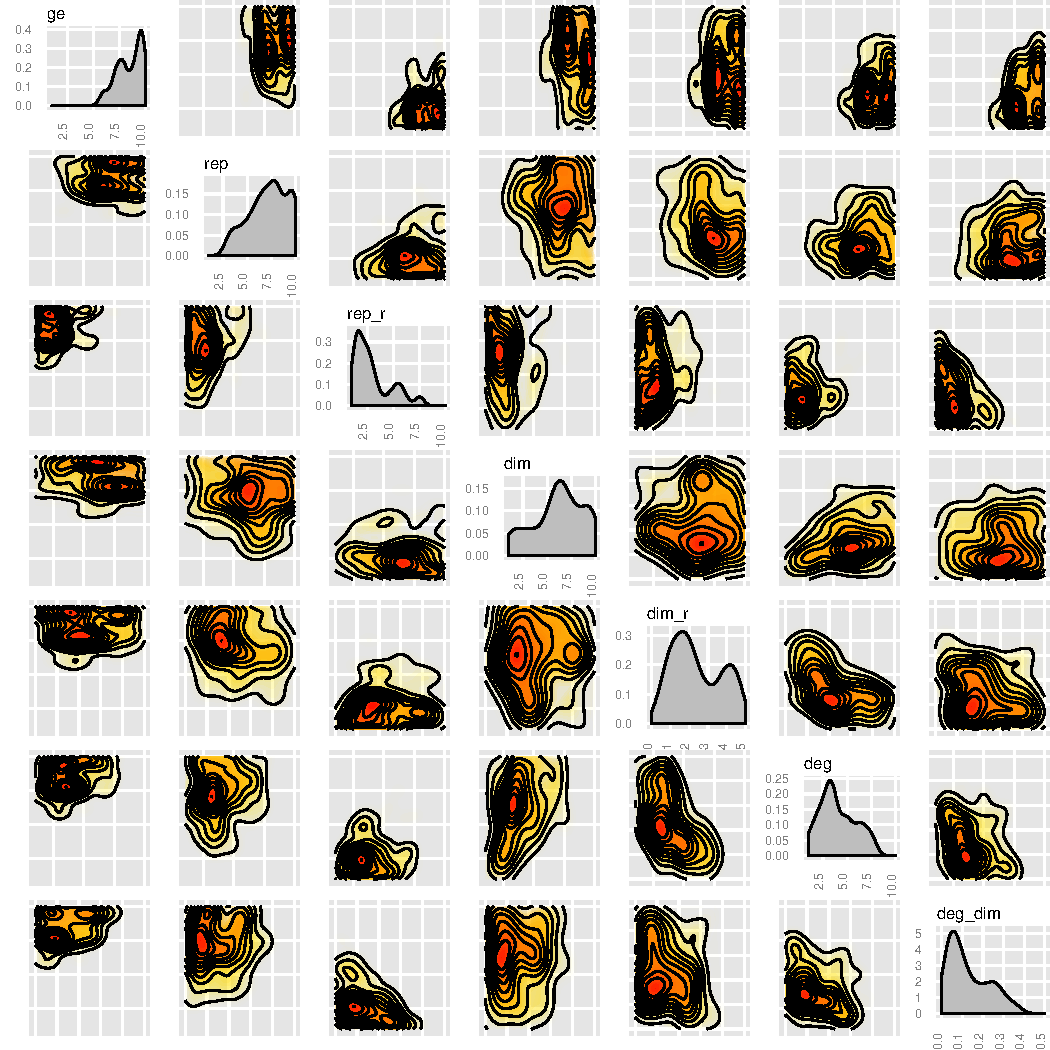
\includegraphics[scale=0.7]{chapterModelling/images/posterior_ma_cl_bi.pdf}
\caption{The posterior distribution of the mass action simple toggle switch}
\label{fig:det_std}
\end{figure}

\begin{figure}[p]
\centering
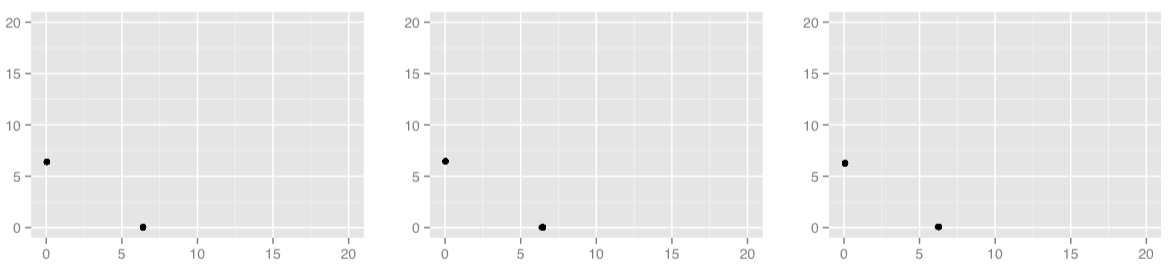
\includegraphics[scale=0.4]{chapterModelling/images/ma_cl_bi_phase_plot.png}
\caption{A sample of the phase plots produced from the final population of the mass action simple toggle switch.}
\label{fig:det_std_phase}
\end{figure}

\begin{figure}[p]
\centering
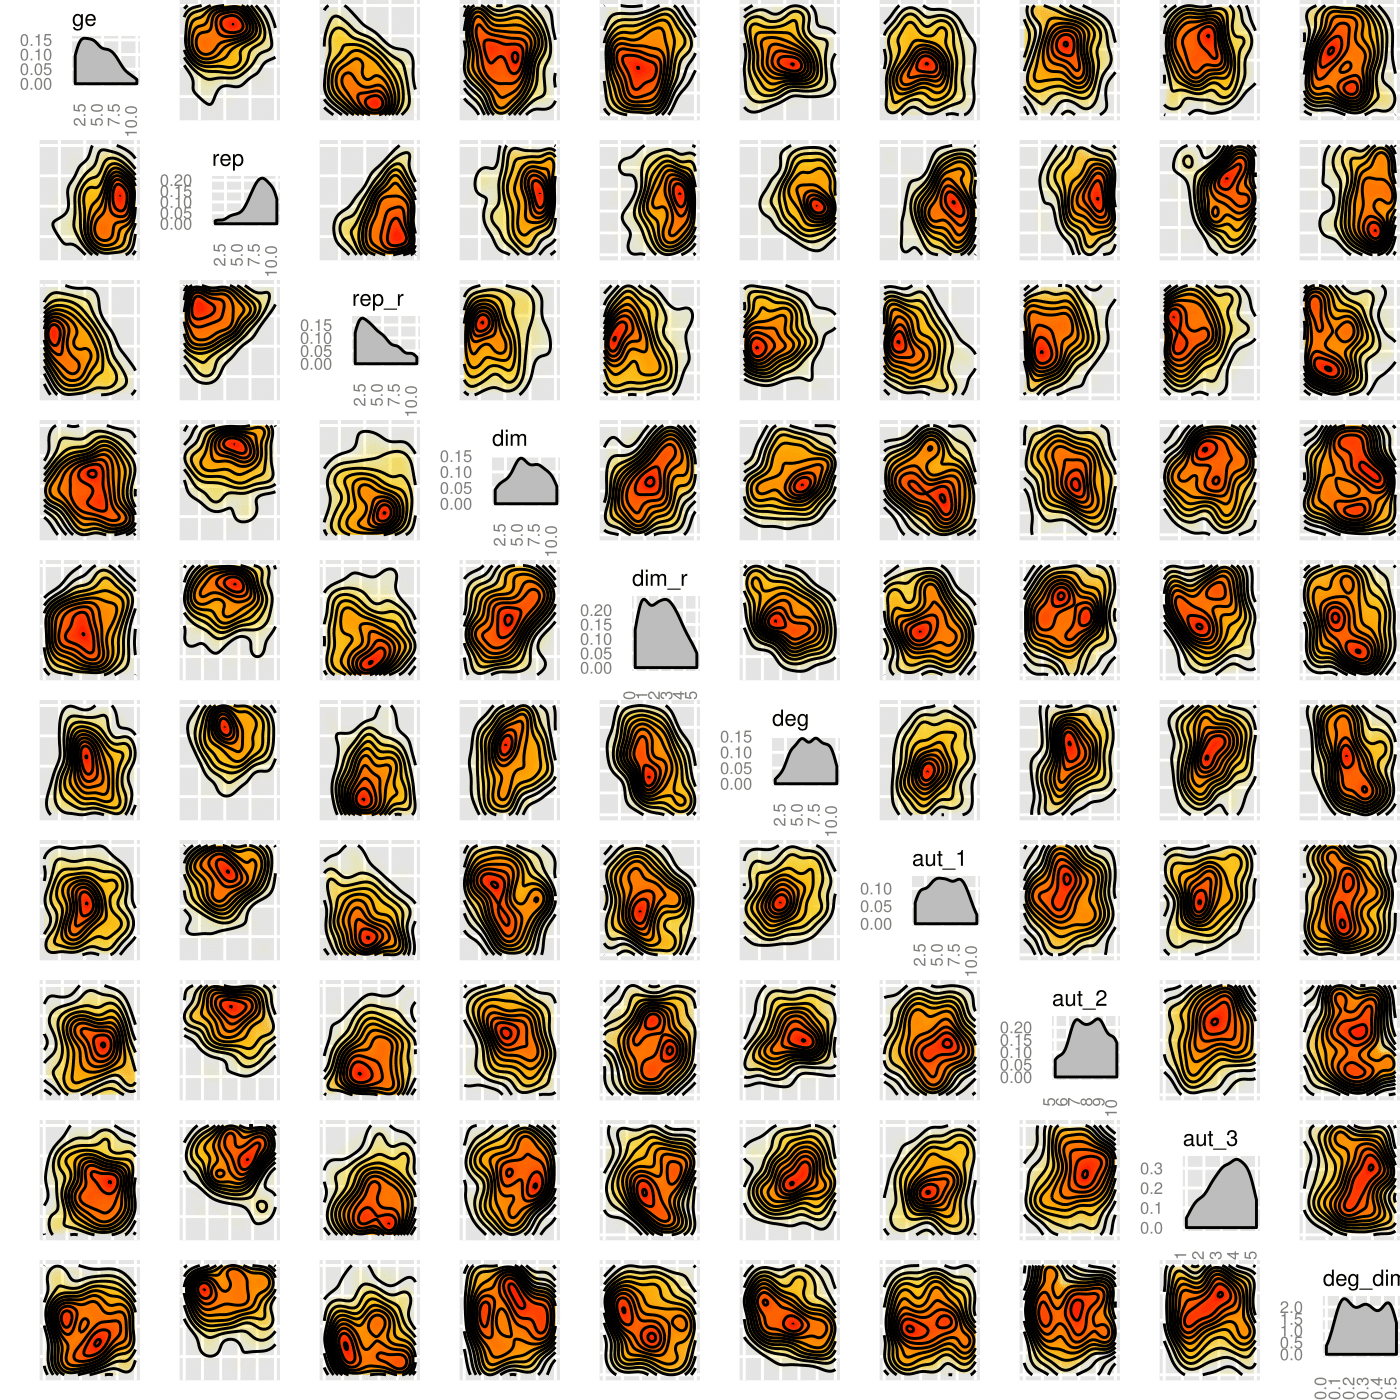
\includegraphics[scale=0.7]{chapterModelling/images/posterior_ma_dp_bi.pdf}
\caption{The posterior distribution of the Mass action double positive feedback loop switch}
\label{fig:doub_pos}
\end{figure}

\begin{figure}[p]
\centering
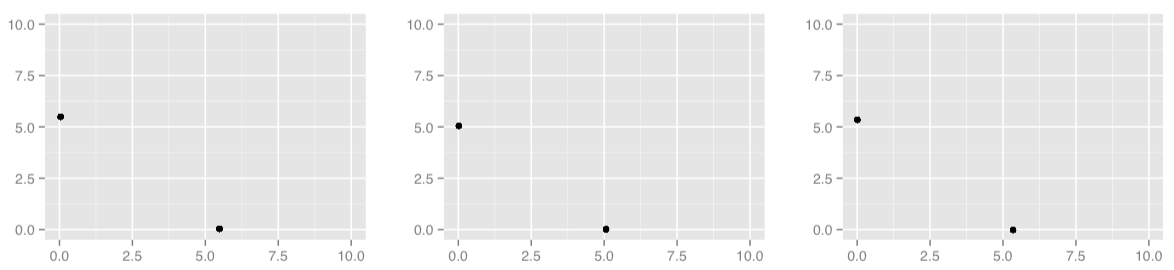
\includegraphics[scale=0.4]{chapterModelling/images/ma_dp_bi_phase_plot.png}
\caption{A sample of the phase plots produced from the final population of the mass action double positive feedback toggle switch.}
\label{fig:det_dp_phase}
\end{figure}

In order to directly compare the robustness of the two models, we used the algorithm outlined in the Methods as a measure of how wide each posterior is given the priors. The results are shown in Figure~\ref{fig:robust_std_doubpos}. 

\begin{figure}[p]
\centering
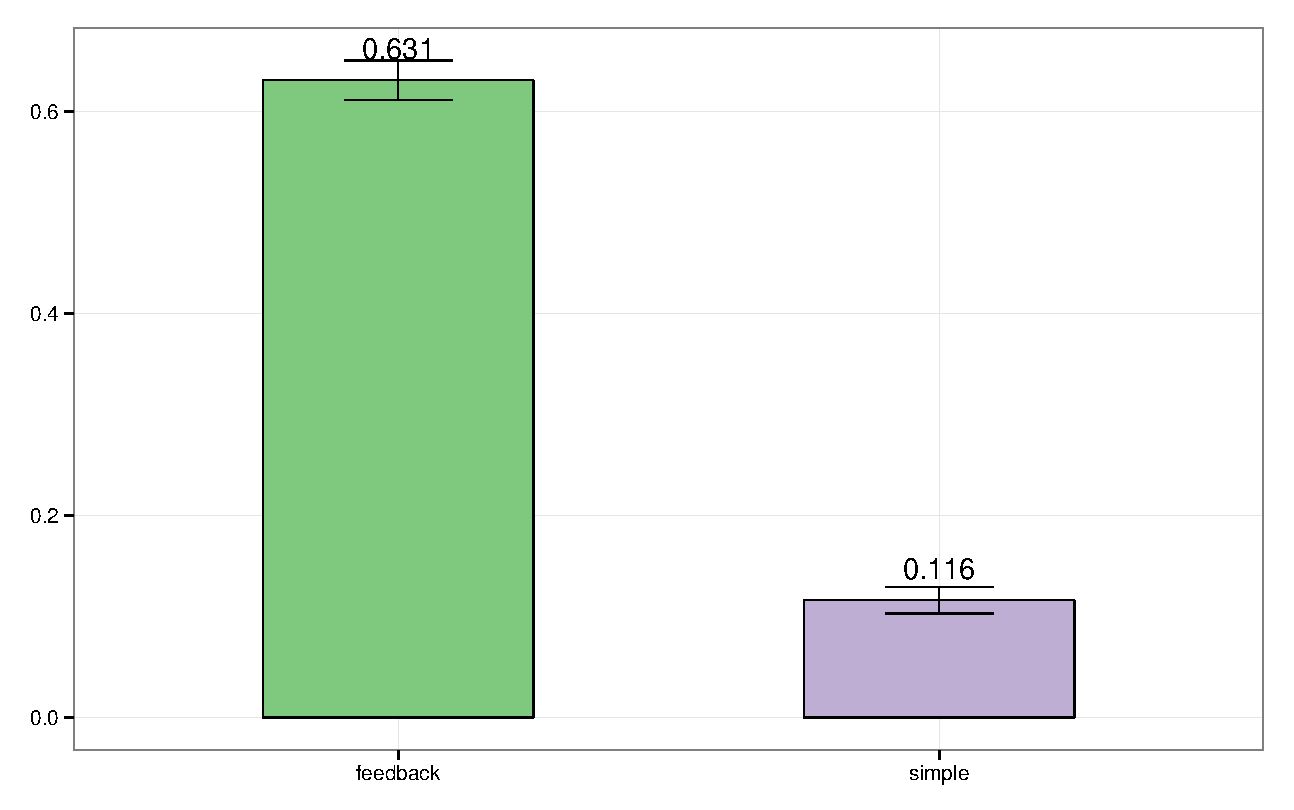
\includegraphics[scale=0.5]{chapterModelling/images/robustness_comparison.pdf}
\caption[The robustness of the double positive and the simple switch mass action models]{The switch with double positive autoregulation is more robust to parameter fluctuations that the simple switch. This is evident from the fact that the switch with added feedback has a larger posterior distribution under which it is bistable, compare to the simple switch. Robustness was calculated using a Monte Carlo accept reject algorithm. }
\label{fig:robust_std_doubpos}
\end{figure}
As seen in Figure~\ref{fig:robust_std_doubpos}, the toggle switch with double positive autoregulation is more robust than the simple switch with no feedback. Adding positive feedback loops to the model allows it to be bistable over a greater range of parameter values. This indicates that small fluctuations in parameters in the cellular environment will not flip the switch and thus makes it more suitable for use in synthetic biological applications where spontaneous and undesired switching might be detrimental. 


%-%-%-%-%-%-%-%-%-%-%%-%-%-%-%-%-%-%-%-%%-%-%-%-%-%-%-%-%-%-%-%-%-%-%-%-%-%-%-%-%-%-%-%-%-%-%-%-%-%
%\newpage
%\subsection{Munsky-Khammash stochastic Gardner switch}
%
%For our next example we selected the Munksy-Khammash toggle switch ~\autocite{Munsky:2008kl}. In this study the authors used a stochastic version of the genetic toggle switch and found it to be bistable for a set of parameter values. We used this to test Stability Checker in the stochastic case.  
%
%\begin{table}[ht!]
%\centering
%\caption{Munsky-Khammash reaction list}
%\label{tab:munsk_reac}
%\begin{tabular}{cccc}
%$R_1$                       & $R_2$ & $R_3$ & $R_4$ \\
%$\oslash \rightarrow s_1$ & $s_1 \rightarrow \oslash$  & $\oslash \rightarrow s_2$ & $s_2 \rightarrow \oslash$  \\
%$w_1 = \frac{a_1}{1+s_2^{\beta}}$                            & $w_2 = s_1$     & $w_3 = \frac{a_2}{1+s_1^{\gamma}} $     & $w_4 = s_2$\\
%$a_1 = 16$ && $a_2 = 50$  \\
%$\beta = 1$ && $\gamma = 2.5$   
%\end{tabular}
%\end{table}
%\newpage
%\begin{figure}[ht!]
%\centering
%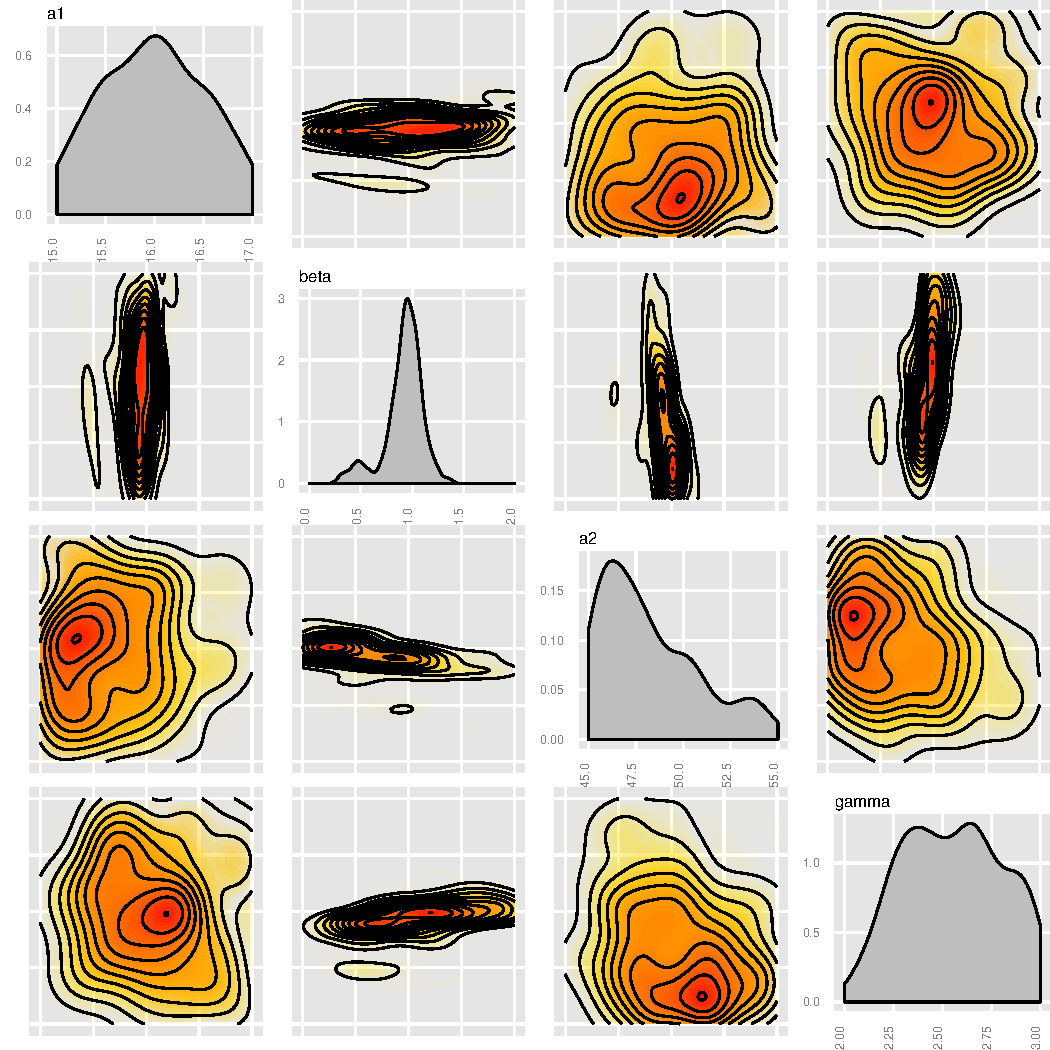
\includegraphics[scale=0.7]{chapterModelling/images/Gardner/Stoch/posterior_100p.pdf}
%\caption{}
%\label{fig:stch_gard}
%\end{figure}
%
%\begin{table}[ht!]
%\centering
%\caption{Munsky-Khammash stochastic switch priors}
%\label{tab:gard_st}
%\begin{tabular}{cccc|cc}
%\multicolumn{4}{c|}{Parameters} & \multicolumn{2}{c}{Species} \\ %\hline
%$a_1$   & $\beta$   & $a_2$   & $\gamma$  &   $s_1$    &       $s_2$   \\
%15-17   &   0-2     &  45-55  &    2-3    &   0-100    &       0-100   
%\end{tabular}
%\end{table}
%
%These values agree with the ones used by the authors to produce a bistable switch.
%
%\begin{figure}[ht!]
%\centering
%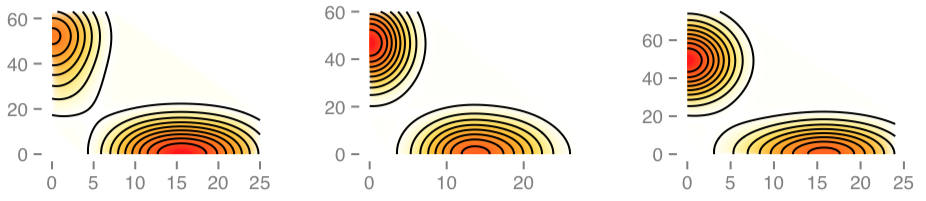
\includegraphics[scale=0.4]{chapterModelling/images/Gardner/Stoch/phase_plots.png}
%\caption{A sample of the phase plots produced from the final population of the Munsky-Khammash switch.}
%\label{fig:stch_gard_phase}
%\end{figure}
%


\newpage
\section{Discussion}

Here we presented a methodology, StabilityChecker, which can identify the region of parameter space that can produce the stability of choice. We demonstrated its use on some known models and extracted stability and robustness information from them. We compared the stability profile of the Gardner toggle switch when modelled deterministically and stochastically in order to uncover the differences that arise from the addition of noise in the modelling. We found that the stochastic model showed increased robustness to noise.

We then applied StabilityChecker to the Lu switches in order to uncover the design principles that make a switch bistable versus tristable. We found that the gene expression parameters were critical for making a tristable switch bistable. This would be in agreement with the dynamics of a tristable switch, in which the third steady state occurs when there is a deadlock situation between the two proteins. When there are small numbers of both proteins involved, one represses the production of the other resulting in both promoters being repressed \autocite{Ma:2012dt}. Given our result we can extrapolate that a higher rate of protein production eliminates the possibility of this deadlock situation happening. Once a promoter is free to produce protein it will produce it in a fast enough rate so that that protein dominates the system and represses the antagonizing promoter before it has the chance to repress it. This dynamic would explain the fact that when all the priors remained the same but gene expression was increased by an order of magnitude, the tristable switch became bistable. 

We also applied StabilityChecker to a synthetic biology design problem. We used two models of the switch, one simple model consisting of two mutually repressive transcription factors and a model with added double positive auto-regulation. Comparing the two models, both capable of bistable behaviour, using StabilityChecker we found that the model with added double positive feedback loops is more robust to parameter fluctuations. This makes it a better candidate for building new synthetic devices based on the toggle switch design. We identified the parameter region within which this models are bistable, information that is important when building such a device in the lab. In the future, by selecting the system components accordingly, the parameter values can be adjusted \textit{in vivo}. For example, the parameter value corresponding to the translation initiation rate can be chosen by selecting the appropriate RBS sequence which given a nucleotide sequence will produce the desired rate \autocite{Holtz:2010bm}, a method developed by Salis \autocite{Salis:2009gk}. Another method to tweak the parameter values \textit{in vivo} is to select the promoter to have the strength corresponding to the levels of gene expression and repression desired. Activity of each promoter can be measured and standardised \autocite{Kelly:2009bj} making this process possible. For a system requiring more than one promoter, these can be efficiently selected from a promoter library using a genetic algorithm created by \textcite{Wu:2011bq}. These standardised interchangeable components with known sequence and activity are what synthetic biology classes as BioBricks \autocite{Kelly:2009bj,Canton:2008fv}. These can be selected and used to construct a desired system and replicate the parameter values found using StabilityChecker.

The methodology we presented here can be applied to a variety of problems as demonstrated. It can be applied to any problem of finding the parameter values that can produce a desired stability between two species. It can be used to design new systems of desired stability and help identify the appropriate parts to use by identifying the rates within which these parts need to operate. It can also be used to examine existing systems and give an insight on the underlying mechanisms that allow for the given stability to occur. 



%%-------------------------------------------------------------%%



\printbibliography



%% --------------------------------------------------------------
%% APPENDIX
%% --------------------------------------------------------------
\chapter{Appendix}
%\addcontentsline{toc}{chapter}{Appendix} 

\section{\acrlong{ode}s}
\subsection{\acrshort{cs-ma}}
$$
\begin{array}{ccl}
\frac {\mathrm{d}\left( {{\mathrm{[A]}} \, \cdot \, {V}_{\mathrm{cell}} } \right) }  {\mathrm{d}{t} }  \; &=& \;  { \, + \, {2} \, \cdot \, {V}_{\mathrm{cell}} \, \cdot \, \left( {{\mathrm{dim\_r}} \, \cdot \, {\mathrm{[A2]}} } \right) } { \, - \, {2} \, \cdot \, {V}_{\mathrm{cell}} \, \cdot \, \left( {{\mathrm{dim}} \, \cdot \, {\mathrm{[A]}} \, \cdot \, {\mathrm{[A]}} } \right) } { \, + \, {V}_{\mathrm{cell}} \, \cdot \, \left( {{\mathrm{geA}} \, \cdot \, {\mathrm{[gA]}} } \right) }{ \, - \, {V}_{\mathrm{cell}} \, \cdot \, \left( {{\mathrm{deg}} \, \cdot \, {\mathrm{[A]}} } \right) } \\ 
 && \\ 
 
\frac {\mathrm{d}\left( {{\mathrm{[gA]}} \, \cdot \, {V}_{\mathrm{cell}} } \right) }  {\mathrm{d}{t} }  \; &=& \;  { \, + \, {V}_{\mathrm{cell}} \, \cdot \, \left( {{\mathrm{rep\_r}} \, \cdot \, {\mathrm{[B2gA]}} } \right) }{ \, - \, {V}_{\mathrm{cell}} \, \cdot \, \left( {{\mathrm{repA}} \, \cdot \, {\mathrm{[gA]}} \, \cdot \, {\mathrm{[B2]}} } \right) } \\ 
 && \\ 
 
\frac {\mathrm{d}\left( {{\mathrm{[B]}} \, \cdot \, {V}_{\mathrm{cell}} } \right) }  {\mathrm{d}{t} }  \; &=& \;  { \, + \, {2} \, \cdot \, {V}_{\mathrm{cell}} \, \cdot \, \left( {{\mathrm{dim\_r}} \, \cdot \, {\mathrm{[B2]}} } \right) } { \, - \, {2} \, \cdot \, {V}_{\mathrm{cell}} \, \cdot \, \left( {{\mathrm{dim}} \, \cdot \, {\mathrm{[B]}} \, \cdot \, {\mathrm{[B]}} } \right) } { \, + \, {V}_{\mathrm{cell}} \, \cdot \, \left( {{\mathrm{geB}} \, \cdot \, {\mathrm{[gB]}} } \right) }{ \, - \, {V}_{\mathrm{cell}} \, \cdot \, \left( {{\mathrm{deg}} \, \cdot \, {\mathrm{[B]}} } \right) } \\ 
 && \\ 
 
\frac {\mathrm{d}\left( {{\mathrm{[gB]}} \, \cdot \, {V}_{\mathrm{cell}} } \right) }  {\mathrm{d}{t} }  \; &=& \;  { \, + \, {V}_{\mathrm{cell}} \, \cdot \, \left( {{\mathrm{rep\_r}} \, \cdot \, {\mathrm{[A2gB]}} } \right) }{ \, - \, {V}_{\mathrm{cell}} \, \cdot \, \left( {{\mathrm{repB}} \, \cdot \, {\mathrm{[gB]}} \, \cdot \, {\mathrm{[A2]}} } \right) } \\ 
 && \\ 
 
\frac {\mathrm{d}\left( {{\mathrm{[A2]}} \, \cdot \, {V}_{\mathrm{cell}} } \right) }  {\mathrm{d}{t} }  \; &=& \;  { \, - \, {V}_{\mathrm{cell}} \, \cdot \, \left( {{\mathrm{dim\_r}} \, \cdot \, {\mathrm{[A2]}} } \right) } { \, + \, {V}_{\mathrm{cell}} \, \cdot \, \left( {{\mathrm{dim}} \, \cdot \, {\mathrm{[A]}} \, \cdot \, {\mathrm{[A]}} } \right) }{ \, - \, {V}_{\mathrm{cell}} \, \cdot \, \left( {{\mathrm{deg\_dim}} \, \cdot \, {\mathrm{[A2]}} } \right) }{ \, + \, {V}_{\mathrm{cell}} \, \cdot \, \left( {{\mathrm{rep\_r}} \, \cdot \, {\mathrm{[A2gB]}} } \right) } \\ 
 && \\ 
 \; && \;  { \, - \, {V}_{\mathrm{cell}} \, \cdot \, \left( {{\mathrm{repB}} \, \cdot \, {\mathrm{[gB]}} \, \cdot \, {\mathrm{[A2]}} } \right) } \\ 
 && \\ 
 
\frac {\mathrm{d}\left( {{\mathrm{[B2]}} \, \cdot \, {V}_{\mathrm{cell}} } \right) }  {\mathrm{d}{t} }  \; &=& \;  { \, - \, {V}_{\mathrm{cell}} \, \cdot \, \left( {{\mathrm{dim\_r}} \, \cdot \, {\mathrm{[B2]}} } \right) }{ \, + \, {V}_{\mathrm{cell}} \, \cdot \, \left( {{\mathrm{dim}} \, \cdot \, {\mathrm{[B]}} \, \cdot \, {\mathrm{[B]}} } \right) }{ \, - \, {V}_{\mathrm{cell}} \, \cdot \, \left( {{\mathrm{deg\_dim}} \, \cdot \, {\mathrm{[B2]}} } \right) } { \, + \, {V}_{\mathrm{cell}} \, \cdot \, \left( {{\mathrm{rep\_r}} \, \cdot \, {\mathrm{[B2gA]}} } \right) } \\ 
 && \\ 
 \; && \;  { \, - \, {V}_{\mathrm{cell}} \, \cdot \, \left( {{\mathrm{repA}} \, \cdot \, {\mathrm{[gA]}} \, \cdot \, {\mathrm{[B2]}} } \right) } \\ 
 && \\ 
 
\frac {\mathrm{d}\left( {{\mathrm{[A2gB]}} \, \cdot \, {V}_{\mathrm{cell}} } \right) }  {\mathrm{d}{t} }  \; &=& \;  { \, - \, {V}_{\mathrm{cell}} \, \cdot \, \left( {{\mathrm{rep\_r}} \, \cdot \, {\mathrm{[A2gB]}} } \right) }{ \, + \, {V}_{\mathrm{cell}} \, \cdot \, \left( {{\mathrm{repB}} \, \cdot \, {\mathrm{[gB]}} \, \cdot \, {\mathrm{[A2]}} } \right) } \\ 
 && \\ 
 
\frac {\mathrm{d}\left( {{\mathrm{[B2gA]}} \, \cdot \, {V}_{\mathrm{cell}} } \right) }  {\mathrm{d}{t} }  \; &=& \;  { \, - \, {V}_{\mathrm{cell}} \, \cdot \, \left( {{\mathrm{rep\_r}} \, \cdot \, {\mathrm{[B2gA]}} } \right) }{ \, + \, {V}_{\mathrm{cell}} \, \cdot \, \left( {{\mathrm{repA}} \, \cdot \, {\mathrm{[gA]}} \, \cdot \, {\mathrm{[B2]}} } \right) } \\ 
 && \\ 
\end{array}
$$

\subsection{\acrshort{dp-ma}}
$$
\begin{array}{ccl}
\frac {\mathrm{d}\left( {{\mathrm{[A]}} \, \cdot \, {V}_{\mathrm{cell}} } \right) }  {\mathrm{d}{t} }  \; &=& \;  { \, - \, {V}_{\mathrm{cell}} \, \cdot \, \left( {{\mathrm{deg}} \, \cdot \, {\mathrm{[A]}} } \right) }{ \, + \, {2} \, \cdot \, {V}_{\mathrm{cell}} \, \cdot \, \left( {{\mathrm{dim\_r}} \, \cdot \, {\mathrm{[A2]}} } \right) }{ \, - \, {2} \, \cdot \, {V}_{\mathrm{cell}} \, \cdot \, \left( {{\mathrm{dim}} \, \cdot \, {\mathrm{[A]}} \, \cdot \, {\mathrm{[A]}} } \right) }{ \, + \, {V}_{\mathrm{cell}} \, \cdot \, \left( {{\mathrm{geA}} \, \cdot \, {\mathrm{[gA]}} } \right) } \\ 
 && \\ 
 \; && \;  { \, + \, {V}_{\mathrm{cell}} \, \cdot \, \left( {{\mathrm{aut\_2}} \, \cdot \, {\mathrm{[A2gA]}} } \right) } \\ 
 && \\ 
 
\frac {\mathrm{d}\left( {{\mathrm{[gA]}} \, \cdot \, {V}_{\mathrm{cell}} } \right) }  {\mathrm{d}{t} }  \; &=& \;  { \, - \, {V}_{\mathrm{cell}} \, \cdot \, \left( {{\mathrm{aut\_1}} \, \cdot \, {\mathrm{[A2]}} \, \cdot \, {\mathrm{[gA]}} } \right) }{ \, + \, {V}_{\mathrm{cell}} \, \cdot \, \left( {{\mathrm{rep\_r}} \, \cdot \, {\mathrm{[B2gA]}} } \right) }{ \, - \, {V}_{\mathrm{cell}} \, \cdot \, \left( {{\mathrm{repA}} \, \cdot \, {\mathrm{[gA]}} \, \cdot \, {\mathrm{[B2]}} } \right) } \\ 
 && \\ 
 \; && \;  { \, + \, {V}_{\mathrm{cell}} \, \cdot \, \left( {{\mathrm{aut\_3}} \, \cdot \, {\mathrm{[A2gA]}} } \right) } \\ 
 && \\ 
 
\frac {\mathrm{d}\left( {{\mathrm{[B]}} \, \cdot \, {V}_{\mathrm{cell}} } \right) }  {\mathrm{d}{t} }  \; &=& \;  { \, + \, {V}_{\mathrm{cell}} \, \cdot \, \left( {{\mathrm{aut\_2}} \, \cdot \, {\mathrm{[B2gB]}} } \right) }{ \, - \, {V}_{\mathrm{cell}} \, \cdot \, \left( {{\mathrm{deg}} \, \cdot \, {\mathrm{[B]}} } \right) }{ \, + \, {2} \, \cdot \, {V}_{\mathrm{cell}} \, \cdot \, \left( {{\mathrm{dim\_r}} \, \cdot \, {\mathrm{[B2]}} } \right) }{ \, - \, {2} \, \cdot \, {V}_{\mathrm{cell}} \, \cdot \, \left( {{\mathrm{dim}} \, \cdot \, {\mathrm{[B]}} \, \cdot \, {\mathrm{[B]}} } \right) } \\ 
 && \\ 
 \; && \;  { \, + \, {V}_{\mathrm{cell}} \, \cdot \, \left( {{\mathrm{geB}} \, \cdot \, {\mathrm{[gB]}} } \right) } \\ 
 && \\ 
 
\frac {\mathrm{d}\left( {{\mathrm{[gB]}} \, \cdot \, {V}_{\mathrm{cell}} } \right) }  {\mathrm{d}{t} }  \; &=& \;  { \, + \, {V}_{\mathrm{cell}} \, \cdot \, \left( {{\mathrm{aut\_3}} \, \cdot \, {\mathrm{[B2gB]}} } \right) }{ \, - \, {V}_{\mathrm{cell}} \, \cdot \, \left( {{\mathrm{aut\_1}} \, \cdot \, {\mathrm{[B2]}} \, \cdot \, {\mathrm{[gB]}} } \right) }{ \, + \, {V}_{\mathrm{cell}} \, \cdot \, \left( {{\mathrm{rep\_r}} \, \cdot \, {\mathrm{[A2gB]}} } \right) } \\ 
 && \\ 
 \; && \;  { \, - \, {V}_{\mathrm{cell}} \, \cdot \, \left( {{\mathrm{repB}} \, \cdot \, {\mathrm{[gB]}} \, \cdot \, {\mathrm{[A2]}} } \right) } \\ 
 && \\ 
 
\frac {\mathrm{d}\left( {{\mathrm{[A2]}} \, \cdot \, {V}_{\mathrm{cell}} } \right) }  {\mathrm{d}{t} }  \; &=& \;  { \, - \, {V}_{\mathrm{cell}} \, \cdot \, \left( {{\mathrm{aut\_1}} \, \cdot \, {\mathrm{[A2]}} \, \cdot \, {\mathrm{[gA]}} } \right) }{ \, + \, {V}_{\mathrm{cell}} \, \cdot \, \left( {{\mathrm{rep\_r}} \, \cdot \, {\mathrm{[A2gB]}} } \right) }{ \, - \, {V}_{\mathrm{cell}} \, \cdot \, \left( {{\mathrm{repB}} \, \cdot \, {\mathrm{[gB]}} \, \cdot \, {\mathrm{[A2]}} } \right) } { \, - \, {V}_{\mathrm{cell}} \, \cdot \, \left( {{\mathrm{dim\_r}} \, \cdot \, {\mathrm{[A2]}} } \right) } \\ 
 && \\ 
 \; && \;  { \, + \, {V}_{\mathrm{cell}} \, \cdot \, \left( {{\mathrm{dim}} \, \cdot \, {\mathrm{[A]}} \, \cdot \, {\mathrm{[A]}} } \right) }{ \, + \, {V}_{\mathrm{cell}} \, \cdot \, \left( {{\mathrm{aut\_3}} \, \cdot \, {\mathrm{[A2gA]}} } \right) } \\ 
 && \\ 
 \; && \;  { \, - \, {V}_{\mathrm{cell}} \, \cdot \, \left( {{\mathrm{deg\_dim}} \, \cdot \, {\mathrm{[A2]}} } \right) } \\ 
 && \\ 
 
\frac {\mathrm{d}\left( {{\mathrm{[B2]}} \, \cdot \, {V}_{\mathrm{cell}} } \right) }  {\mathrm{d}{t} }  \; &=& \;  { \, + \, {V}_{\mathrm{cell}} \, \cdot \, \left( {{\mathrm{aut\_3}} \, \cdot \, {\mathrm{[B2gB]}} } \right) }{ \, - \, {V}_{\mathrm{cell}} \, \cdot \, \left( {{\mathrm{aut\_1}} \, \cdot \, {\mathrm{[B2]}} \, \cdot \, {\mathrm{[gB]}} } \right) }{ \, + \, {V}_{\mathrm{cell}} \, \cdot \, \left( {{\mathrm{rep\_r}} \, \cdot \, {\mathrm{[B2gA]}} } \right) } \\ 
 && \\ 
 \; && \;  { \, - \, {V}_{\mathrm{cell}} \, \cdot \, \left( {{\mathrm{repA}} \, \cdot \, {\mathrm{[gA]}} \, \cdot \, {\mathrm{[B2]}} } \right) }{ \, - \, {V}_{\mathrm{cell}} \, \cdot \, \left( {{\mathrm{dim\_r}} \, \cdot \, {\mathrm{[B2]}} } \right) } { \, + \, {V}_{\mathrm{cell}} \, \cdot \, \left( {{\mathrm{dim}} \, \cdot \, {\mathrm{[B]}} \, \cdot \, {\mathrm{[B]}} } \right) } { \, - \, {V}_{\mathrm{cell}} \, \cdot \, \left( {{\mathrm{deg\_dim}} \, \cdot \, {\mathrm{[B2]}} } \right) } \\ 
 && \\ 
 
\frac {\mathrm{d}\left( {{\mathrm{[B2gA]}} \, \cdot \, {V}_{\mathrm{cell}} } \right) }  {\mathrm{d}{t} }  \; &=& \;  { \, - \, {V}_{\mathrm{cell}} \, \cdot \, \left( {{\mathrm{rep\_r}} \, \cdot \, {\mathrm{[B2gA]}} } \right) }{ \, + \, {V}_{\mathrm{cell}} \, \cdot \, \left( {{\mathrm{repA}} \, \cdot \, {\mathrm{[gA]}} \, \cdot \, {\mathrm{[B2]}} } \right) } \\ 
 && \\ 
 
\frac {\mathrm{d}\left( {{\mathrm{[A2gB]}} \, \cdot \, {V}_{\mathrm{cell}} } \right) }  {\mathrm{d}{t} }  \; &=& \;  { \, - \, {V}_{\mathrm{cell}} \, \cdot \, \left( {{\mathrm{rep\_r}} \, \cdot \, {\mathrm{[A2gB]}} } \right) } { \, + \, {V}_{\mathrm{cell}} \, \cdot \, \left( {{\mathrm{repB}} \, \cdot \, {\mathrm{[gB]}} \, \cdot \, {\mathrm{[A2]}} } \right) } \\ 
 && \\ 
 
\frac {\mathrm{d}\left( {{\mathrm{[B2gB]}} \, \cdot \, {V}_{\mathrm{cell}} } \right) }  {\mathrm{d}{t} }  \; &=& \;  { \, - \, {V}_{\mathrm{cell}} \, \cdot \, \left( {{\mathrm{aut\_3}} \, \cdot \, {\mathrm{[B2gB]}} } \right) } { \, + \, {V}_{\mathrm{cell}} \, \cdot \, \left( {{\mathrm{aut\_1}} \, \cdot \, {\mathrm{[B2]}} \, \cdot \, {\mathrm{[gB]}} } \right) } \\ 
 && \\ 
 
\frac {\mathrm{d}\left( {{\mathrm{[A2gA]}} \, \cdot \, {V}_{\mathrm{cell}} } \right) }  {\mathrm{d}{t} }  \; &=& \;  { \, + \, {V}_{\mathrm{cell}} \, \cdot \, \left( {{\mathrm{aut\_1}} \, \cdot \, {\mathrm{[A2]}} \, \cdot \, {\mathrm{[gA]}} } \right) }{ \, - \, {V}_{\mathrm{cell}} \, \cdot \, \left( {{\mathrm{aut\_3}} \, \cdot \, {\mathrm{[A2gA]}} } \right) } \\ 
 && \\ 
\end{array}
$$
\section{Sequences}
\subsection{pKDL071}


\section{Algorithms}

\subsection{Clustering algorithms}

\subsubsection{Deterministic case}
\begin{algorithm}
\label{alg:DetClustering}
  \caption{Clustering the steady state deterministic simulation results}
 \begin{algorithmic}[1]
    \Statex
      \For{each data point}
      	\If{first point}
      		\State Make first cluster
      		\State cluster counter = 1
      	\Else
      		\For{each cluster}
      			\If{cluster within cluster means $\pm$ delta}      			
      					\State Add to existing cluster
      					\State Update means of clusters
      			\EndIf
      			\If{reached\_end and not assigned to cluster}
      				\State cluster counter +=  1
      				\State Add new cluster
      			\EndIf
      		\EndFor
      	\EndIf
      \EndFor
  \end{algorithmic}
\end{algorithm}
\subsubsection{Stochastic case}
\paragraph{Gap statistic}
\begin{algorithm}
\label{alg:GapStatistic}
\caption{Choosing the optimal number of clusters}
 \begin{algorithmic}[1]
    \Statex
    \Function{Wk}{clusters, cluster\_centres}
    	\For{each cluster}
    		\For{each point in cluster}
    			\State a = matrix norm (cluster\_centre $-$ point)
    		\EndFor
    		\State $dk = \sum((a)^2 )\times (2 \times $ number of points in cluster)
    	\EndFor
    	\State $wk = \frac{ \sum(dk)}{2 \times (number of points in cluster)}$
    	\State \Return wk
    \EndFunction
    %\Statex  
    %\Function{bounding\_box}{data}
    %	\State $xmin, xmax = $ min and max of x axis in data
    %	\State $ymin, ymax = $ min and max of y axis in data
    %	\State \Return $((xmin, xmax), (ymin, ymax)) $
    %\EndFunction
    
    \Statex
    \Function{Gap\_statistic}{data, cutoff}
    	%\State $(xmin, xmax), (ymin, ymax)$ = \Call{bounding\_box}{data}
    	 	\State ks = [1,2,3,4]
    	\For{k in ks}
   			\State cluster\_centres, clusters = \Call{Kmeans}{data, k, cutoff}
   			\State $Wk = \log$(\Call{Wk}{clusters, cluster\_centres})   			
   			\State Create references datasets
   			\For{each references dataset}
			\State cluster\_centres, clusters =  \Call{Kmeans}{data, k, cutoff}
  			\State $BWk = \log$(\Call{Wk}{clusters, cluster\_centres})
   			\EndFor   
   			\State $Wkb = \frac{\sum(BWk)}{10} $	
   			\State $sk = \sqrt{\sum(\frac{(BWk - Wkb)^2}{10})}$	
    	\EndFor
    \State $sk = sk \times \sqrt{1+\frac{1}{B}}$
    \State \Return ks, Wk, Wkb, sk, data\_centres, clusters
    \EndFunction
    \Statex
	\Function{Distance}{data, cutoff}
		    \State ks, logWks, logWkbs, sk, clusters\_means, clusts = \Call{gap\_statistic}{data, cutoff}
		    \State gaps = logWks $-$ logWkbs
		    \State optimum number of clusters = $gaps[i] \geq (gaps[i+1]-sk[i+1])$
	\State \Return cluster\_counter, clusters\_means
	\EndFunction
  \end{algorithmic}
\end{algorithm}
\clearpage
\paragraph{K-means clustering}

\begin{algorithm}
\label{alg:KMeans}
\caption{Clustering stochastic case}
 \begin{algorithmic}[1]
    \Statex
    
    
    \Function{K\-means clustering}{data, k, cutoff}
    	\Statex
    	\Function{Update\_centres}{old\_centres, values}
    		\State centre\_coords =  mean for each dimension
    		\State shift = \Call{getDistance}{centre\_coords, old\_centres}
    		\State \Return shift, centre\_coords
    	\EndFunction
    
    	\Statex
    	\Function{getDistance}{$a, b$}
    		\State $dist = \sqrt{(a[x] - b[x])^2+(a[y] - b[y])^2}$
    		\State \Return $dist$
    	\EndFunction
      
      	\Statex
      	\While{True}
      		\For{each point in data}
      			\For{each cluster}
      				\State $dist = $\Call{getDistance}{point, cluster centre}
      			\EndFor
      			\State Find cluster with minimum distance
      			\State Repopulate clusters
      		\EndFor
      		
      		\Let{biggest\_shift}{0}
      		\For{as many times as there are clusters}
      			\State shift, cluster centres $=$ \Call{Update\_centres}{old\_centres, clusters}
      			\State biggest\_shift =  max between shift, biggest\_shift
      			
      		\EndFor
      		\If{biggest\_shift $\leq$ cutoff}
      			\State break
      		\EndIf
      	\EndWhile
      \State \Return cluster\_centres, clusters
    \EndFunction

  \end{algorithmic}
\end{algorithm}

\clearpage
\end{document}